%% Quanto Custa uma Troca de Chaves Pós-Quântica em um Enlace Li-Fi para IoT?
%% Artigo de disciplina, em estilo tutorial, para leitores que não conhecem
%% Li-Fi nem criptografia pós-quântica.
%%
%% Modelo: SBC (sbc-template.sty, sbc.bst e caption2.sty, distribuídos pela
%% Sociedade Brasileira de Computação e incluídos nesta pasta sem alterações).
%%
%% Compilar:  make        (pdflatex; bibtex; pdflatex x2)
\documentclass[12pt]{article}

\usepackage{sbc-template}
\usepackage[T1]{fontenc}
\usepackage[utf8]{inputenc}
% "provide=*" faz o babel carregar o português a partir dos arquivos .ini, de
% modo que o artigo compila mesmo sem o pacote texlive-lang-portuguese (nesse
% caso só a hifenização fica menos precisa).
\usepackage[english,brazilian,provide=*]{babel}
\usepackage{graphicx,url}
\usepackage{amsmath,amssymb}
\usepackage{booktabs}
\usepackage{tikz}
\usepackage{pgfplots}
\usepgfplotslibrary{groupplots}
\usetikzlibrary{positioning}
\pgfplotsset{compat=1.18}
% números dos eixos no padrão brasileiro: vírgula decimal
\pgfkeys{/pgf/number format/use comma, /pgf/number format/1000 sep={\,}}
\usepackage[hidelinks]{hyperref}

\sloppy
\setlength{\belowcaptionskip}{4pt}   % respiro entre a legenda e a tabela

% Generated by experiments/make_figures_data.py - do not edit.
\makeatletter
\providecommand{\val}[1]{%
  \ifcsname vlc@#1\endcsname\csname vlc@#1\endcsname
  \else\textbf{??#1??}\fi}
\expandafter\gdef\csname vlc@BIKEL1Air100k\endcsname{303}
\expandafter\gdef\csname vlc@BIKEL1Bytes\endcsname{3114}
\expandafter\gdef\csname vlc@BIKEL1Cpu\endcsname{538{,}6}
\expandafter\gdef\csname vlc@BIKEL1CpuRaw\endcsname{538.588}
\expandafter\gdef\csname vlc@BIKEL1Cross\endcsname{0{,}06}
\expandafter\gdef\csname vlc@BIKEL1CrossEn\endcsname{0.06}
\expandafter\gdef\csname vlc@BIKEL1CrossKbpsRaw\endcsname{56}
\expandafter\gdef\csname vlc@BIKEL1Symbols\endcsname{20}
\expandafter\gdef\csname vlc@BitsPerSymbol\endcsname{1275}
\expandafter\gdef\csname vlc@BytesRatio\endcsname{24{,}5}
\expandafter\gdef\csname vlc@ClassicMcEliece348864Air100k\endcsname{23770}
\expandafter\gdef\csname vlc@ClassicMcEliece348864Bytes\endcsname{261216}
\expandafter\gdef\csname vlc@ClassicMcEliece348864Cpu\endcsname{12795{,}5}
\expandafter\gdef\csname vlc@ClassicMcEliece348864CpuRaw\endcsname{12795.469}
\expandafter\gdef\csname vlc@ClassicMcEliece348864Cross\endcsname{0{,}19}
\expandafter\gdef\csname vlc@ClassicMcEliece348864CrossEn\endcsname{0.19}
\expandafter\gdef\csname vlc@ClassicMcEliece348864CrossKbpsRaw\endcsname{186}
\expandafter\gdef\csname vlc@ClassicMcEliece348864Symbols\endcsname{1640}
\expandafter\gdef\csname vlc@DataSubcarriers\endcsname{255}
\expandafter\gdef\csname vlc@ExAirMs\endcsname{151{,}4}
\expandafter\gdef\csname vlc@ExAirPct\endcsname{97}
\expandafter\gdef\csname vlc@ExBitsAir\endcsname{1152}
\expandafter\gdef\csname vlc@ExBitsFrag\endcsname{1088}
\expandafter\gdef\csname vlc@ExCpuPct\endcsname{3}
\expandafter\gdef\csname vlc@ExCyc\endcsname{820\,590}
\expandafter\gdef\csname vlc@ExCycDecaps\endcsname{428\,167}
\expandafter\gdef\csname vlc@ExCycKeygen\endcsname{392\,423}
\expandafter\gdef\csname vlc@ExFrags\endcsname{13}
\expandafter\gdef\csname vlc@ExFragsCt\endcsname{6}
\expandafter\gdef\csname vlc@ExFragsEk\endcsname{7}
\expandafter\gdef\csname vlc@ExFrameMs\endcsname{11{,}52}
\expandafter\gdef\csname vlc@ExRetxPct\endcsname{1}
\expandafter\gdef\csname vlc@ExSpeedup\endcsname{31}
\expandafter\gdef\csname vlc@ExSurvival\endcsname{0{,}989}
\expandafter\gdef\csname vlc@ExTotalMs\endcsname{156{,}3}
\expandafter\gdef\csname vlc@ExTx\endcsname{13{,}14}
\expandafter\gdef\csname vlc@FragBestClean\endcsname{128}
\expandafter\gdef\csname vlc@FragBestNoisy\endcsname{32}
\expandafter\gdef\csname vlc@FragFixedPenalty\endcsname{67}
\expandafter\gdef\csname vlc@FragKiloPenalty\endcsname{2309}
\expandafter\gdef\csname vlc@HQC128Air100k\endcsname{617}
\expandafter\gdef\csname vlc@HQC128Bytes\endcsname{6682}
\expandafter\gdef\csname vlc@HQC128Cpu\endcsname{1263{,}5}
\expandafter\gdef\csname vlc@HQC128CpuRaw\endcsname{1263.538}
\expandafter\gdef\csname vlc@HQC128Cross\endcsname{0{,}05}
\expandafter\gdef\csname vlc@HQC128CrossEn\endcsname{0.05}
\expandafter\gdef\csname vlc@HQC128CrossKbpsRaw\endcsname{49}
\expandafter\gdef\csname vlc@HQC128Symbols\endcsname{42}
\expandafter\gdef\csname vlc@MLKEM1024Air100k\endcsname{303}
\expandafter\gdef\csname vlc@MLKEM1024Bytes\endcsname{3136}
\expandafter\gdef\csname vlc@MLKEM1024Cpu\endcsname{12{,}6}
\expandafter\gdef\csname vlc@MLKEM1024CpuRaw\endcsname{12.577}
\expandafter\gdef\csname vlc@MLKEM1024Cross\endcsname{2{,}41}
\expandafter\gdef\csname vlc@MLKEM1024CrossEn\endcsname{2.41}
\expandafter\gdef\csname vlc@MLKEM1024CrossKbpsRaw\endcsname{2407}
\expandafter\gdef\csname vlc@MLKEM1024Symbols\endcsname{20}
\expandafter\gdef\csname vlc@MLKEM512Air100k\endcsname{151}
\expandafter\gdef\csname vlc@MLKEM512Bytes\endcsname{1568}
\expandafter\gdef\csname vlc@MLKEM512Cpu\endcsname{4{,}9}
\expandafter\gdef\csname vlc@MLKEM512CpuRaw\endcsname{4.884}
\expandafter\gdef\csname vlc@MLKEM512Cross\endcsname{3{,}10}
\expandafter\gdef\csname vlc@MLKEM512CrossEn\endcsname{3.10}
\expandafter\gdef\csname vlc@MLKEM512CrossKbpsRaw\endcsname{3100}
\expandafter\gdef\csname vlc@MLKEM512Symbols\endcsname{10}
\expandafter\gdef\csname vlc@MLKEM768Air100k\endcsname{221}
\expandafter\gdef\csname vlc@MLKEM768Bytes\endcsname{2272}
\expandafter\gdef\csname vlc@MLKEM768Cpu\endcsname{8{,}0}
\expandafter\gdef\csname vlc@MLKEM768CpuRaw\endcsname{8.035}
\expandafter\gdef\csname vlc@MLKEM768Cross\endcsname{2{,}75}
\expandafter\gdef\csname vlc@MLKEM768CrossEn\endcsname{2.75}
\expandafter\gdef\csname vlc@MLKEM768CrossKbpsRaw\endcsname{2754}
\expandafter\gdef\csname vlc@MLKEM768Symbols\endcsname{15}
\expandafter\gdef\csname vlc@McElieceAirS\endcsname{24}
\expandafter\gdef\csname vlc@McElieceCt\endcsname{96}
\expandafter\gdef\csname vlc@McElieceEkKiB\endcsname{255}
\expandafter\gdef\csname vlc@PosCentreBerExp\endcsname{-8}
\expandafter\gdef\csname vlc@PosCentreMs\endcsname{42}
\expandafter\gdef\csname vlc@PosCentreSnr\endcsname{25}
\expandafter\gdef\csname vlc@PosEdgeBer\endcsname{3{,}2\times 10^{-3}}
\expandafter\gdef\csname vlc@PosEdgeMs\endcsname{1214}
\expandafter\gdef\csname vlc@PosEdgeS\endcsname{1{,}2}
\expandafter\gdef\csname vlc@PosEdgeSnr\endcsname{18{,}5}
\expandafter\gdef\csname vlc@PosRatio\endcsname{29}
\expandafter\gdef\csname vlc@PosSnrDrop\endcsname{6{,}5}
\expandafter\gdef\csname vlc@RoleApCpu\endcsname{2{,}3}
\expandafter\gdef\csname vlc@RoleApUp\endcsname{768}
\expandafter\gdef\csname vlc@RoleNodeCpu\endcsname{4{,}9}
\expandafter\gdef\csname vlc@RoleNodeUp\endcsname{800}
\expandafter\gdef\csname vlc@RoleSaving\endcsname{52}
\expandafter\gdef\csname vlc@X25519Air100k\endcsname{23}
\expandafter\gdef\csname vlc@X25519Bytes\endcsname{64}
\expandafter\gdef\csname vlc@X25519Cpu\endcsname{6{,}5}
\expandafter\gdef\csname vlc@X25519CpuRaw\endcsname{6.534}
\expandafter\gdef\csname vlc@X25519Cross\endcsname{0{,}36}
\expandafter\gdef\csname vlc@X25519CrossEn\endcsname{0.36}
\expandafter\gdef\csname vlc@X25519CrossKbpsRaw\endcsname{356}
\expandafter\gdef\csname vlc@X25519Symbols\endcsname{1}
\makeatother
   % gerado por experiments/make_figures_data.py
% Autores e instituição, no formato do modelo SBC.
% Gerado por configurar.py -- prefira rodar o script a editar à mão.
\newcommand{\autores}{Matheus de Oliveira Saldanha\inst{1}, Nicácio De Mattos Cerioni Silva\inst{1}}
\newcommand{\instituicao}{Universidade Estadual de Campinas\\
  Campinas -- SP -- Brasil
  \email{matheus.saldanha@dac.unicamp.br, n218335@dac.unicamp.br}}
% Onde o leitor encontra o código (frase usada no fim da Introdução).
\newcommand{\repositorio}{em github.com/zinho02/lifi-kem/settings}
    % autores e instituição (gerado por configurar.py)

\newcommand{\SK}{\mathsf{SK}}
\newcommand{\ek}{\mathsf{ek}}
\newcommand{\dk}{\mathsf{dk}}
\newcommand{\ct}{\mathsf{ct}}

\title{Quanto Custa uma Troca de Chaves Pós-Quântica\\
em um Enlace Li-Fi para IoT?}

\author{\autores}

\address{\instituicao}

\begin{document}

\maketitle

\begin{abstract}\selectlanguage{english}%
Li-Fi can connect IoT sensors through the light of LED lamps, but the key
exchange that protects such links must migrate to post-quantum algorithms,
whose messages are about $25$ times larger. This paper asks what costs more in
an ML-KEM key exchange over Li-Fi: computing or transmitting. We couple a
validated ML-KEM implementation to a simulation of a Li-Fi room and separate
the two costs. Transmission dominates: both times are equal only at
$\val{MLKEM512CrossEn}$\,Mbit/s, nearly an order of magnitude above low-cost
Li-Fi platforms, and ML-KEM-512 needs even less computation than X25519.
Because corrupted packets are resent, the exchange takes $\val{PosCentreMs}$\,ms
under the lamp and $\val{PosEdgeMs}$\,ms near the wall. Algorithms should
therefore be chosen by message size.
\end{abstract}

\begin{resumo}
O Li-Fi conecta sensores de IoT pela luz de LEDs, mas a troca de
chaves que protege esses enlaces precisa migrar para algoritmos pós-quânticos,
cujas mensagens são cerca de $25$ vezes maiores. Este artigo pergunta o que
custa mais em uma troca de chaves ML-KEM por Li-Fi: calcular ou transmitir.
Ligamos uma implementação validada do ML-KEM a uma sala Li-Fi simulada e
separamos os dois custos. A transmissão domina: os tempos só se igualam
a $\val{MLKEM512Cross}$\,Mbit/s, bem acima das plataformas Li-Fi de baixo custo, e o
ML-KEM-512 exige menos processamento do que a X25519. Como pacotes corrompidos são reenviados, a troca leva
$\val{PosCentreMs}$\,ms sob a luminária e $\val{PosEdgeMs}$\,ms junto à parede.
O algoritmo deve ser escolhido pelo tamanho das mensagens.
\end{resumo}

% =====================================================================
% =====================================================================
\section{Introdução}\label{sec:intro}
% =====================================================================

Imagine uma enfermaria em que cada leito tem um pequeno sensor sem fio que
informa a frequência cardíaca e a temperatura do paciente. O rádio poderia
interferir em parte dos equipamentos médicos, o Wi-Fi já está congestionado e,
de qualquer forma, a sala é iluminada por lâmpadas de LED no teto. E se essas
lâmpadas pudessem transportar os dados?

Essa é a ideia do \emph{light fidelity}, ou Li-Fi. Uma lâmpada de LED é
modulada milhões de vezes por segundo, rápido demais para alguém perceber, e
essa variação leva os dados até um pequeno sensor de luz em cada
dispositivo~\cite{haas2016lifi}. A tecnologia amadureceu, saindo de
experimentos de laboratório para um padrão, o IEEE 802.11bb, publicado em 2023
como parte da família Wi-Fi~\cite{ieee80211bb}. Ela é especialmente atraente
para a \emph{Internet das Coisas} (IoT): a grande e crescente população de
dispositivos pequenos, baratos e alimentados por bateria, como sensores,
medidores e rastreadores, que medem o mundo e relatam o que encontram. Para
esses dispositivos, o Li-Fi oferece espectro livre em abundância, nenhuma
interferência de rádio e uma infraestrutura que já está instalada no teto.

Como a luz não atravessa paredes, é comum dizer que o Li-Fi é seguro por
natureza. Não é. Qualquer pessoa dentro da sala iluminada recebe exatamente o
mesmo sinal que o dispositivo legítimo~\cite{blinowski2019vlcsec,
arfaoui2020plsvlc}. Uma rede Li-Fi de IoT precisa, portanto, de criptografia
como qualquer outra, e, antes de cifrar qualquer coisa, o sensor precisa
combinar uma chave secreta com o ponto de acesso no teto, por esse mesmo enlace
aberto. Essa etapa chama-se \emph{troca de chaves}.

Hoje, a troca de chaves em dispositivos pequenos é feita quase sempre com um
método de curvas elípticas, como a
X25519~\cite{bernstein2006curve25519,rfc7748}. Ela é rápida e compacta, mas tem
prazo de validade conhecido: um \emph{computador quântico} suficientemente
grande poderia quebrá-la com o algoritmo de Shor~\cite{shor1997}. Essa máquina
ainda não existe, mas isso tranquiliza menos do que parece: um atacante pode
gravar hoje o tráfego cifrado e decifrá-lo anos depois, quando a máquina
existir. Essa ameaça, conhecida como \emph{colher agora, decifrar depois},
pesa mais justamente sobre os dados que a IoT coleta, como registros médicos e
industriais, e sobre dispositivos que ficam instalados por uma década ou
mais~\cite{mosca2018quantum}. Em 2024, o instituto norte-americano de padrões
(NIST) publicou o primeiro padrão de troca de chaves resistente a computadores
quânticos, chamado ML-KEM~\cite{fips203}, e a migração começou.

O novo algoritmo traz um porém de ordem prática. Uma troca de chaves X25519
envia $\val{X25519Bytes}$ bytes; uma troca ML-KEM-512 envia
$\val{MLKEM512Bytes}$ bytes, cerca de $25$ vezes mais. Em uma rede cabeada
rápida, ninguém notaria. Mas enlaces Li-Fi de baixo custo para IoT transportam
apenas algumas centenas de quilobits por
segundo~\cite{galisteo2019openvlc}, e, em um enlace assim, os bytes extras
levam um tempo considerável para serem transmitidos. Enquanto isso, a maior
parte da pesquisa sobre criptografia pós-quântica em dispositivos pequenos
concentrou-se em outro custo: quantos ciclos de processador os algoritmos
exigem~\cite{pqm4,burstinghaus2020pqm}. A única proposta anterior de um sensor
Li-Fi pós-quântico informa quanto tempo a sua troca de chaves leva, mas sem
nenhum modelo do enlace de luz que a transporta~\cite{nurmurodov2025esp32}; por
isso, não consegue dizer para onde vai esse tempo.

Este artigo faz uma única pergunta, simples: \emph{quando um sensor de IoT
realiza uma troca de chaves pós-quântica por Li-Fi, o que demora mais, calcular
ou transmitir?} Para respondê-la, ligamos uma implementação funcional do ML-KEM
a uma simulação de uma sala com Li-Fi e medimos os dois custos, para o ML-KEM e
para vários algoritmos alternativos, em diversas velocidades de enlace e
posições na sala.

A resposta é clara. Nos enlaces que os dispositivos Li-Fi de IoT realmente
usam, a transmissão domina com ampla margem, e o tempo de processador quase não
importa. Isso muda qual algoritmo se deve escolher e em que momento se deve
realizar a troca de chaves.

\subsection{Contribuições}
\begin{enumerate}
\item Definimos a \emph{taxa de cruzamento}, a velocidade do enlace em que
      enviar a troca de chaves leva exatamente o mesmo tempo que calculá-la, e
      mostramos que, para os três níveis de segurança do ML-KEM, ela fica entre
      $\val{MLKEM1024Cross}$ e $\val{MLKEM512Cross}$\,Mbit/s. Isso é quase uma
      ordem de grandeza acima da velocidade das plataformas Li-Fi de baixo
      custo para IoT descritas na literatura. Nesses enlaces, o algoritmo deve
      ser escolhido pelo tamanho das suas mensagens, e não pelo seu custo de
      processamento.
\item Em um processador típico de IoT (ARM Cortex-M4), o ML-KEM-512 precisa de
      $\val{MLKEM512Cpu}$\,ms de processamento, \emph{menos} do que os
      $\val{X25519Cpu}$\,ms da X25519 clássica que ele substitui. Migrar para a
      troca de chaves pós-quântica não custa, portanto, nenhum processamento
      adicional nesse tipo de dispositivo; todo o seu preço é tempo de
      transmissão.
\item A troca de chaves precisa entregar mais de mil bytes por um enlace
      imperfeito antes que o sensor possa enviar qualquer outra coisa, e cada
      pacote corrompido tem de ser reenviado. Como a taxa de erro depende de
      quanta luz chega ao sensor, o custo da troca de chaves depende de
      \emph{onde o sensor está na sala}: de $\val{PosCentreMs}$\,ms
      diretamente sob a lâmpada a $\val{PosEdgeMs}$\,ms perto da parede, um
      fator de $\val{PosRatio}$.
\end{enumerate}

Como o artigo une duas áreas que raramente se encontram, as
Seções~\ref{sec:fund-lifi} e~\ref{sec:fund-pqc} apresentam, desde o início, os
fundamentos necessários: primeiro como o Li-Fi transporta dados e por que os
erros dependem da posição; depois como funciona a troca de chaves e por que a
troca pós-quântica é maior. A Seção~\ref{sec:related} revisa os trabalhos
relacionados, a Seção~\ref{sec:model} descreve o cenário e o método, a
Seção~\ref{sec:results} apresenta os resultados, a Seção~\ref{sec:limits}
discute as limitações e a Seção~\ref{sec:conclusion} conclui. Todo o código,
os dados e as figuras estão disponíveis \repositorio.

% =====================================================================
\section{Fundamentos de Li-Fi para a Internet das Coisas}\label{sec:fund-lifi}
% =====================================================================
Esta seção e a próxima foram escritas para leitores que não são especialistas
em comunicações ópticas nem em criptografia. Elas constroem, passo a passo,
todas as ideias necessárias para acompanhar os resultados. Esta trata do lado
da comunicação: o que são os dispositivos de IoT e por que são limitados, como
a luz transporta dados, por que o sinal enfraquece ao longo de uma sala, como
os bits são colocados na luz e o que acontece quando alguns deles chegam
errados. A Tabela~\ref{tab:acronyms} reúne as siglas usadas ao longo do texto.

\begin{table}[!htb]
\caption{Principais siglas e símbolos.}
\label{tab:acronyms}
\centering
\small
\begin{tabular}{ll}
\toprule
termo & significado\\
\midrule
IoT        & Internet das Coisas (pequenos sensores e dispositivos em rede)\\
MCU        & microcontrolador, o pequeno processador de um nó de IoT\\
VLC, Li-Fi & comunicação por luz visível; sua versão em rede\\
LED, PD    & diodo emissor de luz (emissor); fotodiodo (receptor)\\
AP         & ponto de acesso, aqui uma luminária de LED no teto\\
SNR        & relação sinal-ruído, em geral em decibéis (dB)\\
BER        & taxa de erro de bit, fração dos bits recebidos com erro\\
QAM        & modulação de amplitude em quadratura\\
OFDM       & multiplexação por divisão em frequências ortogonais\\
CRC, ARQ   & código de detecção de erros; pedido automático de repetição\\
KEM        & mecanismo de encapsulamento de chaves\\
ML-KEM     & KEM baseado em reticulados, padrão do NIST (FIPS 203)\\
$\ek,\dk,\ct$ & chave de encapsulamento, de desencapsulamento, texto cifrado\\
$R$, $R^{\star}$ & taxa do enlace; taxa de cruzamento (Seção~\ref{sec:cost})\\
\bottomrule
\end{tabular}
\end{table}

\subsection{A Internet das Coisas e suas Limitações}\label{sec:fund-iot}
\emph{Internet das Coisas} (IoT, do inglês \emph{Internet of Things}) é o nome
dado à enorme e crescente população de pequenos dispositivos que medem,
observam ou controlam algo no mundo físico e enviam o resultado por uma rede:
sensores de temperatura e umidade, detectores de presença, medidores
inteligentes, monitores de pacientes, etiquetas de rastreamento em uma fábrica.
Um \emph{nó} típico de IoT tem três partes: um ou mais sensores, um
\emph{microcontrolador} (MCU), que lê os sensores e executa o programa, e um
rádio ou, neste artigo, um transceptor óptico, que o liga a um \emph{ponto de
acesso}. O ponto de acesso encaminha os dados para o restante da rede.

O que distingue um nó de IoT de um celular ou de um notebook é o pouco de que
ele dispõe. A Tabela~\ref{tab:mcus} compara três microcontroladores muito
usados em IoT e em pesquisa com um notebook comum. O processador do nó trabalha
a algumas centenas de megahertz, em vez de vários gigahertz, e tem quilobytes
de memória, em vez de gigabytes. Além disso, costuma ser alimentado por uma
bateria que deve durar meses ou anos; por isso, cada milissegundo que o
processador passa calculando, e cada milissegundo que o transmissor passa
enviando, custa energia.

\begin{table}[!htb]
\caption{Microcontroladores típicos de IoT comparados a um notebook (valores
aproximados).}
\label{tab:mcus}
\centering
\small
\begin{tabular}{lccc}
\toprule
dispositivo & processador & relógio & RAM\\
\midrule
STM32F4 (placa Discovery)  & ARM Cortex-M4 & 168\,MHz & 192\,KB\\
ESP32                      & Xtensa LX6, 2 núcleos & 240\,MHz & 520\,KB\\
Raspberry Pi Pico (RP2040) & ARM Cortex-M0$+$, 2 núcleos & 133\,MHz & 264\,KB\\
\midrule
notebook típico            & x86/ARM, vários núcleos & 3\,GHz & 16\,GB\\
\bottomrule
\end{tabular}
\end{table}

Uma forma útil de pensar no custo de processamento é em \emph{ciclos de
relógio}. Um relógio de $168$\,MHz ``bate'' $168$ milhões de vezes por segundo,
e cada operação simples leva cerca de uma batida. Um algoritmo que precisa de
$C$ ciclos em um processador de frequência $f_{\mathrm{clk}}$ leva, portanto,
\begin{equation}
t = \frac{C}{f_{\mathrm{clk}}}
\label{eq:ciclos}
\end{equation}
segundos. Pela Eq.~\eqref{eq:ciclos}, um algoritmo de $400\,000$ ciclos leva
$400\,000/(168\times10^{6}) \approx 2{,}4$\,ms a $168$\,MHz. A contagem de
ciclos é a forma padrão de comparar programas criptográficos em
microcontroladores porque, ao contrário dos milissegundos, não depende da
frequência configurada. O ARM Cortex-M4, primeiro processador da
Tabela~\ref{tab:mcus}, é a plataforma de referência usual nessas
comparações~\cite{pqm4} e é a que adotamos.

Essas limitações moldam a segurança. Um nó de IoT não consegue executar toda a
pilha de segurança de um navegador, pode permanecer em serviço por uma década e
frequentemente coleta informação sensível: os sinais vitais de um paciente, o
padrão de ocupação de um prédio, o estado de um processo industrial. A
criptografia que ele usa precisa ser barata o bastante para ser executada e
forte o bastante para continuar segura durante toda a vida útil do dispositivo.
É nesse segundo requisito que os computadores quânticos entram na história
(Seção~\ref{sec:fund-quantum}).

\subsection{Comunicação com Luz}\label{sec:fund-light}
A luz visível é radiação eletromagnética, como o rádio, mas de frequência muito
mais alta: cerca de $400$ a $790$\,THz, contra alguns gigahertz do Wi-Fi. A
\emph{comunicação por luz visível} (VLC, \emph{visible light communication})
usa essa luz para transportar dados, e o \emph{Li-Fi} (\emph{light fidelity}) é
a sua versão em rede, na qual cada luminária funciona como um ponto de acesso
sem fio~\cite{haas2016lifi}. O Li-Fi passou recentemente a fazer parte da
família de padrões do Wi-Fi, como IEEE 802.11bb~\cite{ieee80211bb}.

O princípio é simples. Um LED pode ser ligado e desligado, ou ter seu brilho
aumentado e reduzido, milhões de vezes por segundo, muito mais rápido do que o
olho humano percebe; a sala simplesmente parece iluminada de forma constante. O
padrão de variações de brilho codifica os dados, como uma versão muito rápida
de sinalizar com uma lanterna. No receptor, um \emph{fotodiodo}, um pequeno
sensor de luz, produz uma corrente elétrica proporcional à luz que incide sobre
ele, e a eletrônica do receptor converte essa corrente de volta em bits. Esse
esquema chama-se \emph{modulação de intensidade com detecção direta}
(IM/DD)~\cite{kahn1997wireless,ghassemlooy2019owc}. Como o nó não deve iluminar
a sala, o enlace de subida, do nó para o ponto de acesso, normalmente usa luz
infravermelha, que é invisível.

A Tabela~\ref{tab:lifi-wifi} compara Li-Fi e Wi-Fi. Para IoT, três diferenças
importam. O espectro óptico é vasto e não exige licença. A luz não interfere em
equipamentos de rádio, o que é valioso em hospitais, aeronaves e algumas
fábricas. E a luz não atravessa paredes, de modo que uma célula Li-Fi é,
essencialmente, uma sala.

\begin{table}[!htb]
\caption{Li-Fi e Wi-Fi em resumo.}
\label{tab:lifi-wifi}
\centering
\small
\begin{tabular}{lll}
\toprule
 & Wi-Fi & Li-Fi\\
\midrule
portadora            & rádio, 2,4--6\,GHz & luz visível (descida) e infravermelho (subida)\\
espectro             & livre, congestionado & livre, quase sem uso\\
atravessa paredes    & sim & não; uma célula $\approx$ uma sala\\
interferência de rádio & causa e sofre & nenhuma\\
exige visada direta  & não & quase sempre\\
taxas em IoT         & até centenas de Mbit/s & de centenas de kbit/s a Gbit/s\\
\bottomrule
\end{tabular}
\end{table}

É tentador concluir, a partir da última propriedade, que o Li-Fi é seguro por
natureza. Não é. Qualquer pessoa dentro da sala, ou que consiga colocar um
sensor onde a luz chega, recebe exatamente o mesmo sinal que o dispositivo
legítimo~\cite{blinowski2019vlcsec,arfaoui2020plsvlc}. O confinamento reduz
quem pode escutar; não impede a escuta de quem pode. O Li-Fi precisa, portanto,
de criptografia como qualquer outra rede.

\subsection{Como o Sinal Enfraquece ao Longo da Sala}\label{sec:fund-channel}
Um LED não envia sua luz em uma única direção. Ele a espalha em um cone, mais
intenso à frente e mais fraco nas laterais, em um padrão chamado
\emph{lambertiano}. Um receptor diretamente sob a luminária recebe, por isso,
muito mais luz do que um receptor próximo à parede, por dois motivos: está mais
perto e está na parte mais intensa do cone. O modelo padrão desse efeito
fornece a fração da luz emitida que chega ao receptor, chamada \emph{ganho do
canal}~\cite{kahn1997wireless,komine2004vlc}:
\begin{equation}
h = \frac{(m+1)A_{\mathrm{pd}}}{2\pi d^{2}}\cos^{m}(\phi)\cos(\psi),
\qquad 0\le\psi\le\Psi_{\mathrm{fov}}.
\label{eq:gain}
\end{equation}
Cada fator da Eq.~\eqref{eq:gain} tem um significado simples. O termo
$1/d^{2}$ diz que a luz se espalha: dobrar a distância $d$ divide por quatro a
potência recebida, a mesma regra que faz uma lâmpada parecer mais fraca quanto
mais longe se está. O termo $\cos^{m}(\phi)$ descreve o cone: $\phi$ é o ângulo
entre o eixo do LED e a direção do receptor, e o expoente $m$, chamado
\emph{ordem lambertiana}, é maior para um feixe estreito e menor para um feixe
largo. Ele é calculado a partir do ângulo $\Phi_{1/2}$ em que o brilho do LED
cai à metade~\cite{kahn1997wireless}:
\begin{equation}
m = -\frac{\ln 2}{\ln\cos\Phi_{1/2}}.
\label{eq:lambert}
\end{equation}
Para o LED deste trabalho, modelado de acordo com ~\cite{almoliki2022lci}, com $\Phi_{1/2}=70^{\circ}$, a
Eq.~\eqref{eq:lambert} fornece $m\approx0{,}65$. O termo $\cos(\psi)$ leva em
conta a luz que chega inclinada ao detector, e $A_{\mathrm{pd}}$ é a área do
detector: um detector maior coleta mais luz. Por fim, o receptor só enxerga a
luz que chega dentro do seu campo de visão $\Psi_{\mathrm{fov}}$; fora dele, o
ganho é zero.

A luz recebida nunca é perfeitamente limpa. A luz do sol e de outras lâmpadas
acrescenta uma flutuação aleatória à corrente do fotodiodo (\emph{ruído
shot}), e a própria eletrônica do receptor acrescenta mais (\emph{ruído
térmico}). A qualidade com que o receptor recupera os dados depende de quão
forte é o sinal em comparação com esse ruído, grandeza chamada \emph{relação
sinal-ruído} (SNR). A SNR é quase sempre expressa em decibéis (dB), uma escala
logarítmica em que cada $10$\,dB correspondem a um fator de dez: uma SNR de
$20$\,dB significa que a potência do sinal é $100$ vezes a do ruído, e
$30$\,dB, $1000$ vezes. Para o cenário modelado neste trabalho, o ruído é aproximadamente o mesmo em toda a sala ~\cite{almoliki2022lci}, 
enquanto o sinal segue a Eq.~\eqref{eq:gain}, de modo que a SNR em uma posição $(x,y)$
pode ser escrita em relação à SNR no centro, $\mathrm{SNR}_{c}$:
\begin{equation}
\mathrm{SNR}(x,y) = \mathrm{SNR}_{c} + 20\log_{10}\frac{h(x,y)}{h(0,0)} \ \text{dB},
\label{eq:snr}
\end{equation}
em que o fator $20$ (e não $10$) aparece porque a potência elétrica do sinal é
proporcional ao quadrado da potência óptica
recebida~\cite{kahn1997wireless}. Na sala modelada aqui, a
Eq.~\eqref{eq:snr} indica que a SNR cai $\val{PosSnrDrop}$\,dB, de
$\val{PosCentreSnr}$\,dB sob a luminária para $\val{PosEdgeSnr}$\,dB junto à
parede (Figura~\ref{fig:snr}). Como mostram as próximas subseções, essa queda
aparentemente modesta tem grandes consequências.

\subsection{Dos Bits à Luz: Modulação}\label{sec:fund-mod}
\emph{Modulação} é a regra que transforma bits em um sinal físico. A regra
óptica mais simples, o chaveamento liga-desliga (\emph{on--off keying}), envia
um $1$ como luz e um $0$ como escuro, um bit por intervalo de tempo. Enlaces
mais rápidos enviam vários bits por intervalo usando vários níveis.

A \emph{modulação de amplitude em quadratura} (QAM) leva essa ideia a duas
dimensões. Cada grupo de $b$ bits é mapeado em um de $M=2^{b}$ pontos de uma
grade chamada \emph{constelação}; a Figura~\ref{fig:qam} mostra a 16-QAM, em que
cada ponto representa $4$ bits. O receptor mede um ponto, mas o ruído o desloca
um pouco de onde foi enviado, e o receptor então escolhe o ponto da grade mais
próximo. Se o ruído for grande o bastante para empurrar a medida além da linha
do meio do caminho até um ponto vizinho, ocorre um \emph{erro de símbolo}. Os
rótulos são dispostos em \emph{código de Gray}, de modo que pontos vizinhos
diferem em apenas um bit; assim, o erro de símbolo mais provável corrompe só um
dos $b$ bits. Mais pontos por constelação significam mais bits por símbolo, mas
também pontos mais próximos entre si e, portanto, mais erros para a mesma SNR.
Este artigo usa 32-QAM, que transporta $5$ bits por símbolo.

% Constelação 16-QAM com rótulos de Gray e um ponto recebido com ruído.
\begin{figure}[!htb]
\centering
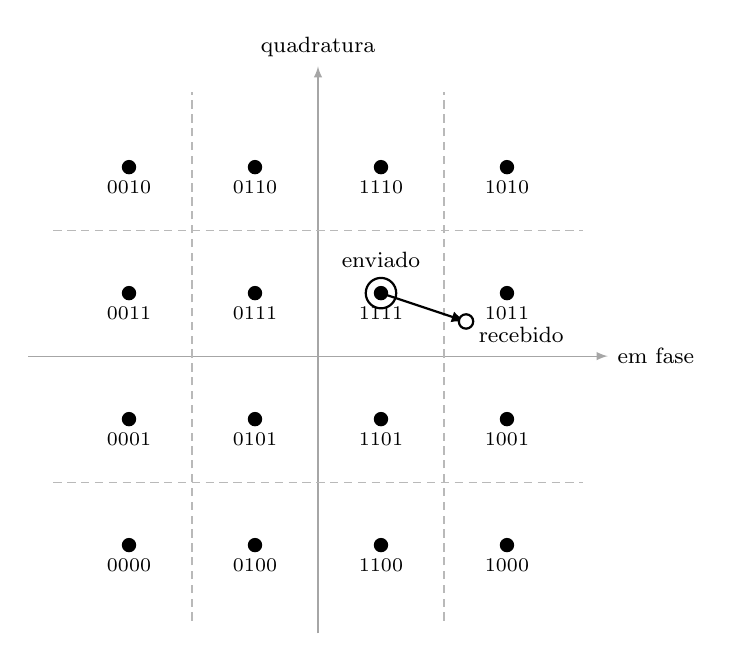
\begin{tikzpicture}[x=0.8cm,y=0.8cm,font=\footnotesize,>=latex]
  % eixos
  \draw[->,gray!70] (-4.6,0) -- (4.6,0) node[right,black] {em fase};
  \draw[->,gray!70] (0,-4.4) -- (0,4.6) node[above,black] {quadratura};
  % fronteiras de decisão
  \foreach \v in {-2,2}{
    \draw[densely dashed,gray!55] (\v,-4.2) -- (\v,4.2);
    \draw[densely dashed,gray!55] (-4.2,\v) -- (4.2,\v);}
  % pontos em código de Gray: amplitude -> rótulo de 2 bits
  \def\lab#1{\ifcase#1 00\or 01\or 11\or 10\fi}
  \foreach \i/\x in {0/-3,1/-1,2/1,3/3}{
    \foreach \j/\y in {0/-3,1/-1,2/1,3/3}{
      \fill (\x,\y) circle (2.6pt);
      \node[below=1.5pt,font=\scriptsize] at (\x,\y) {\lab{\i}\lab{\j}};
    }}
  % ponto enviado, ponto recebido com ruído e o erro
  \draw[black,thick] (1,1) circle (5.5pt);
  \node[anchor=south,fill=white,inner sep=1pt] at (1,1.36) {enviado};
  \draw[->,thick] (1,1) -- (2.35,0.55);
  \fill[white,draw=black,thick] (2.35,0.55) circle (2.6pt);
  \node[anchor=north west,inner sep=1pt] at (2.5,0.52) {recebido};
\end{tikzpicture}
\caption{16-QAM: cada ponto representa 4 bits. As linhas tracejadas são as
fronteiras de decisão. Aqui \texttt{1111} é enviado, o ruído empurra a medida
para além de uma fronteira, e o receptor decide \texttt{1011}. Como os rótulos
seguem um código de Gray, pontos vizinhos diferem em um único bit.}
\label{fig:qam}
\end{figure}


Enviar símbolos QAM um após o outro em alta taxa traz um problema em ambientes
fechados: a luz chega ao receptor por vários caminhos, diretamente e após
refletir nas paredes, e, em altas taxas, essas cópias atrasadas ``borram'' cada
símbolo sobre o seguinte. A \emph{multiplexação por divisão em frequências
ortogonais} (OFDM) evita isso dividindo um fluxo rápido em muitos fluxos lentos,
cada um transportado em sua própria frequência, a \emph{subportadora}, e todos
enviados em paralelo~\cite{armstrong2013ofdm}. Cada fluxo lento quase não é
afetado pelo borrão. A divisão e a recombinação são feitas com a transformada
rápida de Fourier (FFT) e a sua inversa (IFFT), e um curto \emph{prefixo
cíclico}, uma cópia do final de cada símbolo OFDM colocada no seu início,
absorve o borrão que restar.

A luz impõe duas restrições que o rádio não tem. O brilho de um LED é um único
número real e não pode ser negativo. A IFFT normalmente produz um sinal
complexo e bipolar; por isso, são feitos dois ajustes. Primeiro, as $N$
subportadoras, de símbolos $X_0,\dots,X_{N-1}$, são preenchidas em pares
espelhados~\cite{armstrong2013ofdm}:
\begin{equation}
X_{N-k} = X_k^{*}, \qquad X_0 = X_{N/2} = 0,
\label{eq:hermitian}
\end{equation}
em que $X_k^{*}$ é o complexo conjugado de $X_k$. A propriedade da
Eq.~\eqref{eq:hermitian}, chamada \emph{simetria hermitiana}, torna a saída
real. O preço é que apenas metade das $N$ subportadoras transporta dados
independentes, menos as duas que precisam ficar vazias. Segundo, soma-se um
\emph{nível DC} constante para que o sinal fique quase todo positivo, e os
poucos picos que ainda ficarem negativos ou excessivamente altos são
\emph{ceifados} (\emph{clipping}). Esse esquema chama-se \emph{OFDM óptico com
polarização DC} (DCO-OFDM)~\cite{armstrong2013ofdm}, e a Figura~\ref{fig:ofdm}
mostra a cadeia completa.

% Cadeia de transmissão e recepção DCO-OFDM.  TikZ puro.
\begin{figure}[!htb]
\centering
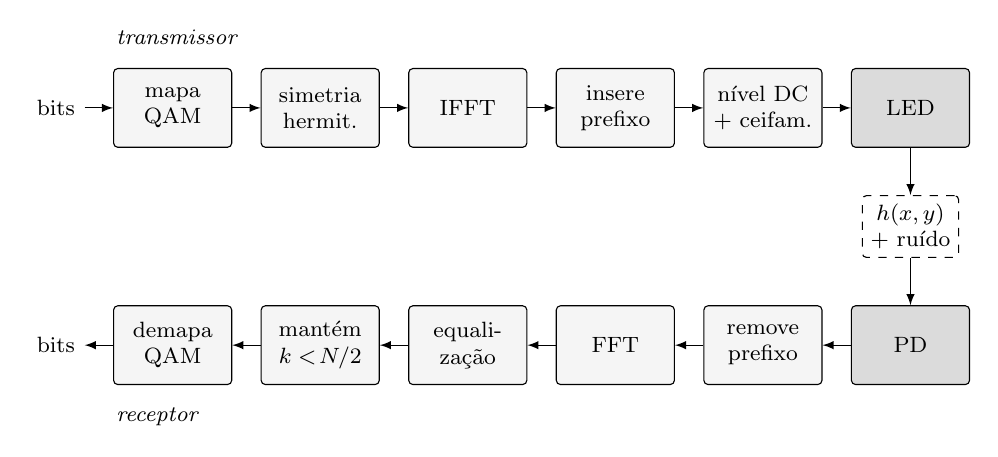
\begin{tikzpicture}[
  font=\footnotesize,
  blk/.style={draw,rounded corners=1.5pt,align=center,inner sep=3pt,
              minimum height=10mm,minimum width=15mm,fill=black!4},
  opt/.style={blk,fill=black!14},
  every path/.style={>=latex,->},
  node distance=3.6mm
]
% ------------------------------ transmissor ------------------------------
\node (bits) {bits};
\node[blk,right=of bits]   (qam)  {mapa\\QAM};
\node[blk,right=of qam]    (herm) {simetria\\hermit.};
\node[blk,right=of herm]   (ifft) {IFFT};
\node[blk,right=of ifft]   (cp)   {insere\\prefixo};
\node[blk,right=of cp]     (dc)   {nível DC\\+ ceifam.};
\node[opt,right=of dc]     (led)  {LED};
\draw (bits) -- (qam);
\draw (qam) -- (herm);
\draw (herm) -- (ifft);
\draw (ifft) -- (cp);
\draw (cp) -- (dc);
\draw (dc) -- (led);
\node[anchor=south west,font=\footnotesize\itshape,inner sep=1pt]
     at ([yshift=2.5mm]qam.north west) {transmissor};

% --------------------------------- canal ---------------------------------
\node[draw,dashed,rounded corners=1.5pt,align=center,inner sep=3pt,
      below=6mm of led] (ch)
     {$h(x,y)$\\$+$ ruído};
\draw (led) -- (ch);

% -------------------------------- receptor --------------------------------
\node[opt,below=6mm of ch]  (pd)   {PD};
\node[blk,left=of pd]       (rcp)  {remove\\prefixo};
\node[blk,left=of rcp]      (fft)  {FFT};
\node[blk,left=of fft]      (eq)   {equali-\\zação};
\node[blk,left=of eq]       (sel)  {mantém\\$k<\!N/2$};
\node[blk,left=of sel]      (dem)  {demapa\\QAM};
\node[left=of dem]          (obits){bits};
\draw (ch) -- (pd);
\draw (pd) -- (rcp);
\draw (rcp) -- (fft);
\draw (fft) -- (eq);
\draw (eq) -- (sel);
\draw (sel) -- (dem);
\draw (dem) -- (obits);
\node[anchor=north west,font=\footnotesize\itshape,inner sep=1pt]
     at ([yshift=-2.5mm]dem.south west) {receptor};
\end{tikzpicture}
\caption{Cadeia DCO-OFDM. A simetria hermitiana da Eq.~\eqref{eq:hermitian}
torna real a saída da IFFT, para que ela possa acionar um LED; o nível DC e o
ceifamento a tornam não negativa. Só $N/2-1$ subportadoras transportam dados, o
que fixa a carga de um símbolo na Eq.~\eqref{eq:bsym}. Os blocos sombreados são
ópticos.}
\label{fig:ofdm}
\end{figure}


Juntando as peças~\cite{armstrong2013ofdm}, conclui-se que cada símbolo
DCO-OFDM transporta
\begin{equation}
B_{\mathrm{sym}} = \left(\tfrac{N}{2}-1\right)\log_2 M \ \text{bits}.
\label{eq:bsym}
\end{equation}
Com $N=512$ subportadoras e 32-QAM, a Eq.~\eqref{eq:bsym} resulta em
$(256-1)\times5 = \val{BitsPerSymbol}$ bits, cerca de $159$ bytes por símbolo
OFDM.

O ceifamento distorce ligeiramente o sinal. Um resultado conhecido como
teorema de Bussgang permite tratar essa distorção como uma pequena e previsível
perda de sinal, de fator $\alpha$, somada a um ruído adicional de potência
$\sigma_c^{2}$~\cite{dimitrov2013information}. Se $\gamma$ é a SNR sem
ceifamento, em escala linear, a SNR efetiva passa a ser
\begin{equation}
\gamma_{\mathrm{ef}} = \frac{\alpha^{2}}{\gamma^{-1} + \sigma_c^{2}}.
\label{eq:gammaeff}
\end{equation}
Para o ceifamento usado aqui, em $\pm3{,}2$ desvios-padrão, $\alpha\approx0{,}999$
e $\sigma_c^{2}\approx1{,}9\times10^{-4}$, de modo que a
Eq.~\eqref{eq:gammaeff} quase não altera a SNR nas condições estudadas.

\subsection{Quando os Bits Chegam Errados: a Taxa de Erro de Bit}\label{sec:fund-ber}
A \emph{taxa de erro de bit} (BER) é a fração dos bits recebidos que estão
errados. Uma BER de $10^{-5}$ significa um bit errado a cada $100\,000$. Ela
depende da SNR e da constelação e, para QAM com código de Gray, é bem
aproximada por~\cite{proakis2008digital}
\begin{equation}
P_b \simeq \frac{\bar{n}\,h_{\mathrm{nn}}}{\log_2 M}\,
           Q\!\left(d_{\min}\sqrt{\gamma_{\mathrm{ef}}/2}\right),
\label{eq:ber}
\end{equation}
em que $\gamma_{\mathrm{ef}}$ é a SNR efetiva da Eq.~\eqref{eq:gammaeff},
$d_{\min}$ é a distância entre pontos vizinhos da constelação, $\bar{n}$ é o
número médio de vizinhos de um ponto e $h_{\mathrm{nn}}$ é o número de bits que
diferem entre vizinhos (cerca de um, graças ao código de Gray). A função
$Q(\cdot)$ é a probabilidade de um ruído gaussiano exceder certo número de
desvios-padrão; o que importa aqui é que ela cai muito depressa à medida que
seu argumento cresce.

Essa queda abrupta é a razão de alguns decibéis fazerem tanta diferença. A
Figura~\ref{fig:snr} aplica as Eqs.~\eqref{eq:snr} e~\eqref{eq:ber} ao longo da
sala. Sob a luminária, a $\val{PosCentreSnr}$\,dB, a BER é de cerca de
$10^{-8}$: um bit errado a cada cem milhões. Junto à parede, apenas
$\val{PosSnrDrop}$\,dB abaixo, ela é de $\val{PosEdgeBer}$, cerca de três bits
errados a cada mil, mais de cem mil vezes maior. Como mostra a
Seção~\ref{sec:results}, essa diferença domina o custo da troca de chaves na
borda da sala.

% SNR e BER ao longo da sala (y = 0), a partir do modelo do enlace.
\begin{figure}[!htb]
\centering
\begin{tikzpicture}
\begin{groupplot}[
  group style={group size=1 by 2, vertical sep=0.6cm, x descriptions at=edge bottom},
  width=0.8\textwidth, height=4.6cm,
  xmin=-2.5, xmax=2.5, grid=both, grid style={gray!18},
  label style={font=\small}, tick label style={font=\footnotesize},
  xlabel={posição do receptor $x$ (m), com $y=0$},
]
\nextgroupplot[ylabel={SNR (dB)}, ymin=17, ymax=26]
  \addplot[black,line width=0.9pt] table[x=x,y=snr_db] {data/handshake_position.dat};
  \node[font=\footnotesize,anchor=north] at (axis cs:0,22.6) {sob a luminária};
  \draw[gray!60,->] (axis cs:0,22.7) -- (axis cs:0,24.7);
  \node[font=\footnotesize,anchor=south west] at (axis cs:-2.45,17.3) {parede};
\nextgroupplot[ymode=log, ylabel={BER}, ymin=1e-9, ymax=1e-2,
  ytick={1e-8,1e-6,1e-4,1e-2}]
  \addplot[black,line width=0.9pt] table[x=x,y=ber] {data/handshake_position.dat};
  \addplot[gray!70,densely dashed,domain=-2.5:2.5] {1e-5};
  \node[font=\footnotesize,anchor=south,gray!40!black] at (axis cs:0,1.2e-5)
    {$10^{-5}$: um bit errado em $100\,000$};
\end{groupplot}
\end{tikzpicture}
\caption{Qualidade do sinal ao longo da sala, pelas Eqs.~\eqref{eq:snr}
e~\eqref{eq:ber}. A SNR cai apenas $\val{PosSnrDrop}$\,dB do centro até a
parede, mas a BER sobe cinco ordens de grandeza, de cerca de
$10^{\val{PosCentreBerExp}}$ para $\val{PosEdgeBer}$.}
\label{fig:snr}
\end{figure}


\subsection{Pacotes, Verificação de Erros e Retransmissão}\label{sec:fund-arq}
Enlaces reais não enviam um único fluxo longo de bits; enviam \emph{pacotes}.
Uma mensagem longa demais para um pacote é cortada em \emph{fragmentos}, cada
um enviado com um pequeno \emph{cabeçalho} que indica qual fragmento é e
carrega um código de verificação. O código usado quase universalmente, a
verificação de redundância cíclica (CRC), é um código curto calculado a partir
do conteúdo do fragmento. O receptor o recalcula; se os dois valores diferem,
ao menos um bit foi corrompido, e o fragmento é descartado.

Um fragmento descartado precisa ser enviado de novo. A forma mais simples de
organizar isso é o \emph{pedido automático de repetição do tipo
pare-e-espere} (ARQ \emph{stop-and-wait}): o emissor transmite um fragmento e
aguarda uma curta confirmação; se ela não chega, envia o mesmo fragmento outra
vez. Cada retransmissão custa tempo de transmissão.

A probabilidade de um fragmento chegar intacto decorre diretamente da BER. Se
cada um dos seus $n$ bits está errado, de forma independente, com probabilidade
$P_b$, todos os $n$ bits estão certos com
probabilidade~\cite{bertsekas1992data}
\begin{equation}
P_{\mathrm{ok}} = (1-P_b)^{n}.
\label{eq:psurv}
\end{equation}
Um fragmento com $128$ bytes de dados e $8$ bytes de cabeçalho tem
$n = 8\times136 = 1088$ bits. Pela Eq.~\eqref{eq:psurv}, com $P_b=10^{-5}$ ele
sobrevive com probabilidade $0{,}989$, e retransmissões são raras. Com
$P_b=10^{-3}$, sobrevive com probabilidade $(0{,}999)^{1088}\approx0{,}34$:
dois em cada três fragmentos se perdem e precisam ser reenviados. Esse é o
mecanismo por trás do efeito da posição mostrado na Seção~\ref{sec:results}, e
ele também explica por que fragmentos menores ajudam em um enlace ruim: menos
bits por fragmento significam mais chance de cada um chegar inteiro.

% =====================================================================
\section{Fundamentos da Troca de Chaves Pós-Quântica}\label{sec:fund-pqc}
% =====================================================================
Esta seção explica, desde o início, por que um nó de IoT precisa combinar uma
chave, como isso é feito hoje, por que os computadores quânticos ameaçam esse
processo e como funciona o novo padrão do NIST, o ML-KEM, cujas mensagens são
muito maiores.

\subsection{Por que Dois Dispositivos Precisam de uma Chave em Comum}\label{sec:fund-sym}
A maior parte dos dados que um sensor envia é protegida com criptografia
\emph{simétrica}: emissor e receptor possuem a mesma chave secreta, e a mesma
chave serve para cifrar e para decifrar. Cifras simétricas como o AES, ou a
família leve Ascon, padronizada pelo NIST em 2025 para dispositivos
restritos~\cite{sp800232}, são rápidas e baratas o bastante para qualquer
microcontrolador.

A criptografia simétrica deixa uma pergunta em aberto: como os dois
dispositivos passam a ter a mesma chave? Um nó tirado da caixa e instalado em
uma enfermaria nunca ``conheceu'' o ponto de acesso com o qual vai conversar, e
tudo o que um diz ao outro trafega por um enlace que qualquer pessoa na sala
pode observar (Seção~\ref{sec:fund-light}). Enviar a chave às claras a
revelaria. Esse é o \emph{problema da distribuição de chaves}, e ele é
resolvido pela \emph{criptografia de chave pública}. Uma analogia conhecida é a
do cadeado aberto. Suponha que o ponto de acesso queira receber um segredo: ele
envia ao nó um cadeado \emph{aberto} e guarda a única chave. O nó coloca um
segredo recém-escolhido em uma caixa, fecha o cadeado e devolve a caixa.
Qualquer um pode ver o cadeado e a caixa em trânsito, mas só o ponto de acesso
consegue abri-la. Os algoritmos de chave pública usados neste artigo
funcionam, em essência, como esse cadeado.

\subsection{Troca de Chaves Clássica: Diffie--Hellman e X25519}\label{sec:fund-dh}
A troca de chaves usada hoje em quase toda parte é a de Diffie--Hellman. Uma
analogia popular usa tintas. As duas partes começam com uma cor comum e
pública. Cada uma mistura a ela uma cor secreta e envia a mistura à outra. Em
seguida, cada uma acrescenta a sua própria cor secreta ao que recebeu. As duas
terminam com a mesma cor final, a cor comum mais os dois segredos, enquanto um
observador que viu apenas as duas misturas não consegue separar os segredos,
porque ``desmisturar'' tinta é difícil.

Na versão matemática, ``misturar'' é uma operação sobre os pontos de uma curva
elíptica, e ``desmisturar'' é o \emph{problema do logaritmo discreto em curvas
elípticas}, para o qual não se conhece algoritmo clássico eficiente. A variante
mais usada, a X25519~\cite{bernstein2006curve25519,rfc7748}, é compacta: cada
parte envia um único valor de 32 bytes, de modo que a troca completa movimenta
$\val{X25519Bytes}$ bytes. Ela também é barata o bastante para rodar em um
microcontrolador. Há duas décadas esse é o modo padrão de pequenos dispositivos
combinarem uma chave.

\subsection{A Ameaça Quântica}\label{sec:fund-quantum}
Um \emph{computador quântico} processa informação usando efeitos da mecânica
quântica e, para alguns problemas específicos, pode ser dramaticamente mais
rápido do que qualquer computador comum. Um desses problemas é exatamente o que
protege a troca de Diffie--Hellman. Em 1994, Peter Shor mostrou que um
computador quântico suficientemente grande resolveria com eficiência tanto a
fatoração de inteiros quanto o logaritmo discreto~\cite{shor1997}, o que
quebraria o RSA, o Diffie--Hellman e a X25519.

A criptografia simétrica resiste muito melhor. O melhor ataque quântico
conhecido contra ela, o algoritmo de Grover, apenas acelera a busca exaustiva
da chave por uma raiz quadrada, e o remédio usual, usar chaves mais longas,
como o AES de 256 bits, é simples. O ponto fraco de uma implantação de IoT na
era quântica não é, portanto, a cifração dos dados, e sim a \emph{troca de
chaves} que a prepara.

Não existe hoje um computador quântico grande o bastante para executar o
algoritmo de Shor contra chaves reais, e as estimativas de quando existirá
variam muito. Por que se preocupar agora? Porque o atacante não precisa do
computador quântico no momento do ataque. Ele pode gravar hoje uma sessão
cifrada, armazená-la e decifrá-la quando a máquina estiver disponível: é a
ameaça conhecida como \emph{colher agora, decifrar depois} (\emph{harvest now,
decrypt later}). Mosca~\cite{mosca2018quantum} resume o prazo resultante em uma
desigualdade simples. Seja $x$ o número de anos durante os quais os dados
precisam permanecer confidenciais, $y$ o número de anos necessários para trocar
a criptografia dos dispositivos já instalados e $z$ o número de anos até
existir um computador quântico de grande porte. Então, se
\begin{equation}
x + y > z,
\label{eq:mosca}
\end{equation}
os dados coletados hoje já estão expostos. Em IoT, os dois termos do lado
esquerdo da Eq.~\eqref{eq:mosca} são grandes: dados médicos e industriais
muitas vezes precisam permanecer privados por muitos anos, e dispositivos
embarcados, uma vez instalados, podem ficar uma década sem atualização. É por
isso que a migração para a criptografia pós-quântica é urgente justamente para
o tipo de dispositivo considerado neste artigo.

\emph{Criptografia pós-quântica} significa algoritmos comuns, que rodam em
processadores comuns, projetados para resistir a ataques de computadores
quânticos, além dos clássicos. Ela não exige hardware quântico, apenas software
novo. O NIST conduziu uma competição aberta, de vários anos, para selecionar
esses algoritmos; a Tabela~\ref{tab:nist} resume seus marcos.

\begin{table}[!htb]
\caption{Principais marcos da padronização pós-quântica do NIST.}
\label{tab:nist}
\centering
\small
\begin{tabular}{ll}
\toprule
ano & marco\\
\midrule
2016 & o NIST abre a chamada pública por algoritmos pós-quânticos\\
2022 & CRYSTALS-Kyber é selecionado para estabelecimento de chaves\\
2024 & publicação do FIPS 203 (ML-KEM, derivado do Kyber)~\cite{fips203}\\
     & e do FIPS 204 (ML-DSA), para assinaturas~\cite{fips204}\\
2025 & HQC é selecionado como segundo KEM, baseado em códigos~\cite{nisthqc2025};\\
     & SP 800-227, com recomendações de uso de KEMs~\cite{sp800227}\\
\bottomrule
\end{tabular}
\end{table}

\subsection{Mecanismos de Encapsulamento de Chaves}\label{sec:fund-kem}
O substituto pós-quântico do Diffie--Hellman é apresentado na forma de um
\emph{mecanismo de encapsulamento de chaves} (KEM, \emph{key-encapsulation
mechanism})~\cite{cramer2003kem,sp800227}. Um KEM é o cadeado da
Seção~\ref{sec:fund-sym} em versão precisa. Ele é formado por três algoritmos:
\begin{itemize}
\item $\textsc{KeyGen}() \to (\ek, \dk)$ fabrica um cadeado novo e a sua chave:
      uma \emph{chave de encapsulamento} pública $\ek$ e uma \emph{chave de
      desencapsulamento} privada $\dk$;
\item $\textsc{Encaps}(\ek) \to (K, \ct)$ escolhe um segredo aleatório novo $K$
      e o tranca: o \emph{texto cifrado} $\ct$ é a caixa fechada;
\item $\textsc{Decaps}(\dk, \ct) \to K$ abre a caixa e recupera $K$.
\end{itemize}
Em uma troca de chaves, uma parte executa \textsc{KeyGen} e envia $\ek$; a
outra executa \textsc{Encaps}, guarda $K$ e devolve $\ct$; a primeira executa
\textsc{Decaps} e passa a ter o mesmo $K$. Duas diferenças em relação ao
Diffie--Hellman serão importantes adiante. As duas mensagens são objetos
diferentes, de tamanhos diferentes, e as duas partes realizam quantidades
diferentes de trabalho. Ambas afetam o comportamento da troca em um enlace de
capacidade limitada.

Um KEM precisa continuar seguro mesmo contra um atacante capaz de injetar
textos cifrados de sua autoria e observar como o receptor reage. O nome formal
dessa propriedade é segurança IND-CCA2. Os KEMs baseados em reticulados a
obtêm com uma técnica chamada transformada de
Fujisaki--Okamoto~\cite{fujisaki1999,hofheinz2017fo}: ao abrir uma caixa, o
\textsc{Decaps} refaz a caixa a partir do que encontrou dentro dela e verifica
se o resultado é idêntico à caixa recebida. Se um único bit for diferente, a
caixa foi adulterada ou danificada.

O que o \textsc{Decaps} faz em seguida é uma decisão de projeto sutil, mas
importante. A escolha óbvia, devolver um erro, seria um equívoco: um atacante
que possa enviar muitos textos cifrados modificados e observar quais produzem
erro aprende algo com cada resposta, e ataques exatamente desse tipo já
quebraram sistemas reais~\cite{bleichenbacher1998}. O ML-KEM usa, em vez disso,
a \emph{rejeição implícita}: quando a verificação falha, ele devolve
silenciosamente um valor de aparência aleatória, calculado a partir de uma
semente secreta e do texto cifrado~\cite{fips203}. O atacante não aprende nada,
e as duas partes legítimas simplesmente ficam com chaves diferentes, o que
percebem na primeira tentativa de usá-las. Em um enlace ruidoso, essa é também
a última linha de defesa contra erros de transmissão que escapem ao código de
verificação da Seção~\ref{sec:fund-arq}.

Um KEM, sozinho, não confirma a identidade de ninguém; ele apenas estabelece um
segredo. Por isso, o NIST recomenda alimentar uma \emph{função de derivação de
chaves} com esse segredo e com as mensagens trocadas~\cite{sp800227}. Uma
função de derivação de chaves é construída a partir de uma \emph{função de
hash}, um algoritmo que transforma qualquer entrada em uma ``impressão
digital'' de tamanho fixo, de modo que entradas diferentes produzem, na
prática, impressões diferentes. Derivar a chave de sessão do segredo do KEM e
de uma impressão digital de toda a conversa amarra a chave àquela troca
específica, de forma que uma troca adulterada gera uma chave inútil.

\subsection{O ML-KEM e a Dificuldade das Equações com Ruído}\label{sec:fund-mlkem}
O ML-KEM (\emph{Module-Lattice-based KEM}), padronizado como FIPS 203 e
derivado do CRYSTALS-Kyber~\cite{fips203,bos2018kyber}, apoia-se em um problema
fácil de enunciar e, até onde se sabe, difícil de resolver mesmo com um
computador quântico: resolver um sistema de equações lineares em que cada
equação recebeu um pequeno erro.

Um exemplo de brinquedo transmite a ideia. Trabalhando módulo $17$, suponha
que lhe informem
\begin{equation}
3s_1 + 5s_2 \equiv 2, \qquad 7s_1 + 2s_2 \equiv 9 \pmod{17}.
\label{eq:toy}
\end{equation}
O sistema da Eq.~\eqref{eq:toy} pode ser resolvido por eliminação, exatamente
como na álgebra escolar, e dá $s_1=2$, $s_2=6$. Suponha agora que cada lado
direito tenha sido alterado por um pequeno valor aleatório, $-1$, $0$ ou $+1$,
e que você não saiba qual. A eliminação multiplica e subtrai as equações, e
multiplica e subtrai junto os erros ocultos; depois de alguns passos, os erros
cresceram até o tamanho dos próprios números, e a resposta perde o sentido. Com
duas incógnitas ainda é possível testar todas as possibilidades, mas no
ML-KEM-512 o segredo tem $512$ incógnitas, muito além de qualquer busca
exaustiva. Esse é o problema do \emph{aprendizado com erros} (LWE,
\emph{learning with errors}), introduzido por Regev~\cite{regev2009lwe}; o
ML-KEM usa uma variante estruturada, o LWE em \emph{módulos} (MLWE), que
preserva a dificuldade e torna a aritmética muito mais
rápida~\cite{langlois2015mlwe}.

No ML-KEM, os números são substituídos por polinômios de 256 coeficientes, com
toda a aritmética feita módulo $q=3329$. A chave pública contém uma matriz
aleatória $\mathbf{A}$, de dimensão $k\times k$, formada por esses polinômios,
e um vetor~\cite{fips203}
\begin{equation}
\mathbf{t} = \mathbf{A}\mathbf{s} + \mathbf{e},
\label{eq:mlwe}
\end{equation}
em que o segredo $\mathbf{s}$ e o erro $\mathbf{e}$ têm coeficientes pequenos.
A Eq.~\eqref{eq:mlwe} é o sistema com ruído da Eq.~\eqref{eq:toy} em escala
muito maior: recuperar $\mathbf{s}$ a partir de $(\mathbf{A},\mathbf{t})$ é o
problema difícil. A matriz $\mathbf{A}$ nunca é enviada de fato: os dois lados
a regeneram a partir de uma semente $\rho$ de 32 bytes. A dimensão $k$ define o
nível de segurança. A Tabela~\ref{tab:mlkem} lista os três conjuntos de
parâmetros do padrão, que visam às categorias de segurança 1, 3 e 5 do NIST,
aproximadamente tão difíceis de quebrar quanto o AES-128, o AES-192 e o
AES-256.

\begin{table}[!htb]
\caption{Conjuntos de parâmetros do ML-KEM (FIPS 203). Tamanhos em bytes.
$\delta$ é a probabilidade de uma troca honesta falhar por razões
criptográficas.}
\label{tab:mlkem}
\centering
\small
\begin{tabular}{lcccccc}
\toprule
conjunto & $k$ & $(\eta_1;\eta_2)$ & $(d_u;d_v)$ & $|\ek|$ & $|\ct|$ & $\delta$\\
\midrule
ML-KEM-512  & 2 & (3; 2) & (10; 4) & \phantom{1}800  & \phantom{1}768  & $2^{-138{,}8}$\\
ML-KEM-768  & 3 & (2; 2) & (10; 4) & 1184 & 1088 & $2^{-164{,}8}$\\
ML-KEM-1024 & 4 & (2; 2) & (11; 5) & 1568 & 1568 & $2^{-174{,}8}$\\
\bottomrule
\end{tabular}
\end{table}

Os tamanhos das mensagens decorrem dessa estrutura, e vale a pena deduzi-los,
porque eles determinam todos os resultados deste artigo. A chave de
encapsulamento carrega $\mathbf{t}$, que são $k$ polinômios de 256
coeficientes; cada coeficiente é um número menor que $3329$ e precisa de 12
bits. Somando a semente de 32 bytes, obtém-se~\cite{fips203}
\begin{equation}
|\ek| = \frac{256\times12}{8}\,k + 32 = 384k + 32 \ \text{bytes},
\label{eq:eksize}
\end{equation}
ou seja, $800$ bytes no ML-KEM-512, em que $k=2$. O texto cifrado é formado por
$k+1$ polinômios \emph{comprimidos}, dos quais se guardam apenas $d_u$ ou $d_v$
bits por coeficiente~\cite{fips203}:
\begin{equation}
|\ct| = 32\,(d_u k + d_v) \ \text{bytes},
\label{eq:ctsize}
\end{equation}
o que dá $768$ bytes no ML-KEM-512. As Eqs.~\eqref{eq:eksize}
e~\eqref{eq:ctsize} reproduzem todas as linhas da Tabela~\ref{tab:mlkem}. O
segredo compartilhado $K$ tem sempre $32$ bytes. As probabilidades de falha
$\delta$ da tabela são tão pequenas, abaixo de uma em $10^{41}$, que na prática
uma troca honesta nunca falha por razões criptográficas. Em um enlace ruidoso,
toda falha é uma falha de transmissão.

Embora as chaves sejam grandes, o cálculo é rápido. A multiplicação de
polinômios é feita com a transformada numérica (NTT), uma versão da FFT que
trabalha com números inteiros, e toda a aleatoriedade e todo o hash usam o
SHAKE, da família SHA-3~\cite{fips202}. Em um ARM Cortex-M4, uma geração de
chaves do ML-KEM-512 leva menos de $400\,000$ ciclos, o que, pela
Eq.~\eqref{eq:ciclos}, corresponde a cerca de $2{,}3$\,ms a
$168$\,MHz~\cite{pqm4}.

\subsection{Por que as Trocas de Chaves Pós-Quânticas São Grandes}\label{sec:fund-size}
Colocar os números lado a lado torna visível a tensão central deste artigo.
Uma troca X25519 movimenta $\val{X25519Bytes}$ bytes; uma troca ML-KEM-512
movimenta $\val{MLKEM512Bytes}$, cerca de $25$ vezes mais. A diferença não é uma
ineficiência do projeto: um problema de equações com ruído só é difícil se
contiver muitas equações, e cada equação contribui com coeficientes que
precisam ser transmitidos. A criptografia baseada em reticulados troca tamanho
por velocidade. Ela é maior do que a de curvas elípticas no enlace, mas, como
mostra a Seção~\ref{sec:results}, não é mais lenta para calcular em um
microcontrolador.

Outros KEMs pós-quânticos fazem trocas diferentes. Os esquemas \emph{baseados
em códigos} apoiam-se na dificuldade de decodificar um código corretor de erros
aleatório, problema estudado há mais de quarenta anos. O NIST selecionou o HQC
em 2025 como segundo KEM padrão justamente para que um eventual avanço contra
os reticulados não deixasse o mundo sem um padrão~\cite{nisthqc2025}. O BIKE
foi uma alternativa próxima, e o Classic McEliece é o mais conservador de
todos. Seus tamanhos, listados na Tabela~\ref{tab:kems}, têm formatos
incomuns: o HQC-128 e o BIKE-L1 enviam alguns quilobytes em cada sentido,
enquanto o Classic McEliece envia um texto cifrado minúsculo, de 96 bytes, mas
exige uma chave pública de 255 quilobytes. Em um enlace no qual cada byte custa
tempo de transmissão, esses formatos levam a resultados muito diferentes, que
são o assunto do restante do artigo.

% =====================================================================
\section{Trabalhos Relacionados}\label{sec:related}
% =====================================================================
Os trabalhos relevantes para este artigo dividem-se em três grupos: segurança
para comunicação por luz visível, que modela o enlace óptico, mas não a troca
de chaves pós-quântica; criptografia pós-quântica em dispositivos restritos,
que modela o processamento, mas não o enlace; e uma proposta recente que
combina os dois temas.

\subsection{Segurança para Comunicação por Luz Visível}
Os levantamentos de Blinowski~\cite{blinowski2019vlcsec} e de Arfaoui
\emph{et al.}~\cite{arfaoui2020plsvlc} estabelecem que a natureza de difusão do
canal óptico expõe a VLC à escuta dentro da área iluminada e catalogam duas
famílias de contramedidas.

A primeira é a segurança de camada física \emph{sem chaves}, que explora a
geometria do canal para dar ao receptor legítimo uma vantagem sobre o espião,
por meio de formação de feixe, ruído artificial ou argumentos de capacidade de
sigilo~\cite{arfaoui2020plsvlc}. Guo \emph{et al.}~\cite{guo2025skavlc}, por
exemplo, obtêm limites para a capacidade de geração de chave secreta em um
enlace com um único LED, sob a restrição de amplitude do LED, e mostram que uma
taxa de chave positiva se mantém mesmo quando o canal do espião é tão bom
quanto o legítimo. Dang \emph{et al.}~\cite{dang2020qkdvlc} seguem um caminho
óptico-quântico e analisam a distribuição quântica de chaves com variáveis
contínuas sobre VLC em ambientes internos. As duas abordagens geram material de
chave a partir de propriedades físicas do enlace; a primeira depende de uma
vantagem de canal que a instalação precisa garantir, e a segunda, de hipóteses
ópticas muito além dos LEDs comuns.

A segunda família é a \emph{cifração na camada física}, na qual o sinal OFDM é
embaralhado com chaves que mudam a cada quadro. Al-Moliki \emph{et al.} extraem
bits de chave da polaridade do prefixo cíclico~\cite{almoliki2016keygen},
estendem a ideia com mapas caóticos~\cite{almoliki2019chaos} e propõem um
esquema leve e independente do canal para VLC-IoT, que dispensa realimentação
do estado do canal~\cite{almoliki2022lci}; Melki
\emph{et al.}~\cite{melki2019dynamic} descrevem uma cifra OFDM de chave
dinâmica comparável, para rádio. Esses esquemas modelam o canal óptico em
detalhe, mas compartilham uma hipótese: a chave de sessão de longo prazo, da
qual derivam as chaves de cada quadro, é estabelecida previamente por
criptografia de chave pública convencional, e essa troca fica fora do escopo
dos trabalhos. Se for uma troca baseada em curvas elípticas, o esquema inteiro
herda a sua exposição a um futuro adversário quântico. Nenhum desses trabalhos
considera quanto custaria realizar uma troca pós-quântica pelo mesmo enlace,
que é a pergunta tratada aqui.

\subsection{Criptografia Pós-Quântica em Dispositivos Restritos}
A viabilidade dos KEMs baseados em reticulados em microcontroladores é hoje uma
questão resolvida. O projeto pqm4 mantém um ambiente de medição e implementações
otimizadas para o ARM Cortex-M4, a plataforma de referência de fato para
medições de criptografia pós-quântica embarcada~\cite{pqm4}; seus números
colocam uma geração de chaves, um encapsulamento e um desencapsulamento
completos do ML-KEM-512 bem dentro do orçamento de um nó sensor. Chen e
Chou~\cite{chen2021mceliece} mostram que até o Classic McEliece, cuja chave
pública excede a memória RAM da placa-alvo, pode ser executado no mesmo
processador mantendo a chave na memória flash. Bürstinghaus-Steinbach
\emph{et al.}~\cite{burstinghaus2020pqm} integram o Kyber e o SPHINCS$^{+}$ a
uma pilha TLS embarcada em hardware da classe do ESP32, e Segatz e
Al~Hafiz~\cite{segatz2025kyberesp32} aceleram o Kyber no ESP32 usando seus dois
núcleos e seu coprocessador de hash.

Duas observações dessa literatura orientam o nosso método. Primeiro, esses
estudos medem processamento, memória e energia de forma isolada; a rede
aparece, quando aparece, como um enlace rápido, com fio ou por rádio, cujo
tempo de transmissão é desprezível. Essa é justamente a hipótese que o Li-Fi
para IoT quebra. Segundo, detalhes de implementação importam nas comparações:
os ganhos de velocidade relatados em~\cite{segatz2025kyberesp32} para o ESP32
valem para a variante ``90s'' do Kyber, que usa AES e SHA-2, ao passo que o
ML-KEM padronizado usa SHAKE, que o acelerador de hash do ESP32 não implementa.
Por isso, tomamos os tempos de processamento das medições do pqm4 no Cortex-M4,
que cobrem o algoritmo padronizado.

\subsection{Troca de Chaves Pós-Quântica para Li-Fi}
O trabalho mais próximo do nosso é o de Nurmurodov
\emph{et al.}~\cite{nurmurodov2025esp32}, que propõem um nó sensor Li-Fi
baseado no ESP32, o qual estabelece chaves de sessão com um KEM de reticulados
e protege os dados com cifração autenticada. A arquitetura deles e a nossa
coincidem no essencial: uma troca de chaves com KEM, em duas mensagens, pelo
enlace óptico, seguida de cifração simétrica com a chave derivada. A avaliação
deles, porém, não contém camada física. Não se especifica modelo de canal,
modulação, taxa do enlace ou taxa de erro, e o conjunto de parâmetros do KEM é
descrito apenas como ``Kyber-lite''. A latência da troca que eles relatam é,
portanto, um número único, que não pode ser dividido em processamento e
transmissão e que não diz como a troca se comporta quando a taxa do enlace ou a
posição do nó mudam.

Este artigo preenche essa lacuna. Ao acoplar uma implementação validada do
ML-KEM a um modelo explícito do enlace óptico, conseguimos separar os dois
custos, localizar a taxa em que um supera o outro e mostrar como esse
equilíbrio muda ao longo de uma sala.


% =====================================================================
\section{Cenário e Método}\label{sec:model}
% =====================================================================
Esta seção descreve a sala simulada, o protocolo de troca de chaves, a forma de
medir o seu custo e o software que produz os resultados.

% Cenário e troca de chaves.  TikZ puro, sem imagens externas.
\begin{figure}[!htb]
\centering
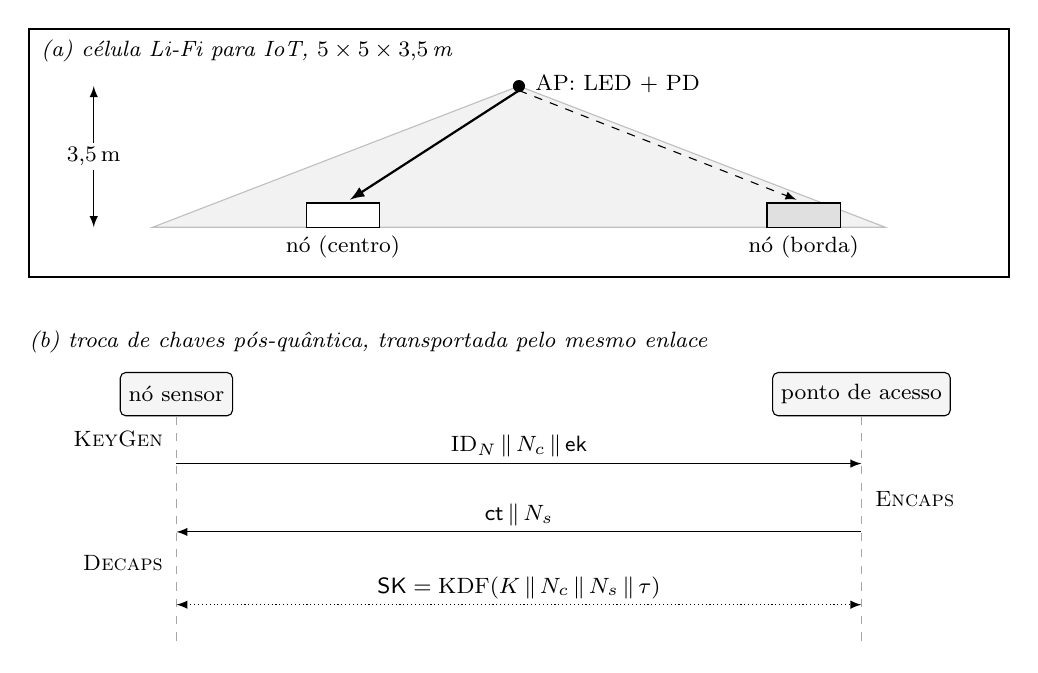
\begin{tikzpicture}[
  x=1.5cm, y=1.4cm,
  font=\footnotesize,
  box/.style={draw,rounded corners=2pt,align=center,inner sep=3pt,
              minimum height=5.5mm,fill=black!4},
  every path/.style={>=latex}
]
% ---------------------------- (a) sala ----------------------------
\begin{scope}
  \def\rw{8.3} \def\rh{2.25}
  \draw[thick] (0,0) rectangle (\rw,\rh);
  \node[anchor=north west,font=\footnotesize\itshape,inner sep=3pt]
       at (0.03,\rh-0.02) {(a) célula Li-Fi para IoT, $5\times5\times3{,}5$\,m};
  \draw[gray!50,fill=gray!10]
     (\rw/2,\rh-0.52) -- (1.05,0.45) -- (\rw-1.05,0.45) -- cycle;
  \fill (\rw/2,\rh-0.52) circle (2.2pt);
  \node[anchor=west,inner sep=4pt] at (\rw/2+0.04,\rh-0.50) {AP: LED $+$ PD};
  \draw[fill=white] (2.35,0.45) rectangle ++(0.62,0.22);
  \node[anchor=north,inner sep=3pt] at (2.66,0.45) {nó (centro)};
  \draw[fill=black!12] (6.25,0.45) rectangle ++(0.62,0.22);
  \node[anchor=north,inner sep=3pt] at (6.56,0.45) {nó (borda)};
  \draw[->,thick]  (\rw/2,\rh-0.56) -- (2.72,0.70);
  \draw[->,dashed] (\rw/2,\rh-0.56) -- (6.50,0.70);
  \draw[<->] (0.55,0.45) -- (0.55,\rh-0.52)
       node[midway,fill=white,inner sep=1.5pt] {$3{,}5$\,m};
\end{scope}
% ----------------------- (b) troca de chaves -----------------------
\begin{scope}[yshift=-4.5cm]
  \def\lx{1.25} \def\rx{7.05} \def\ty{2.15}
  \node[anchor=north west,font=\footnotesize\itshape,inner sep=0pt]
       at (0,\ty+0.58) {(b) troca de chaves pós-quântica, transportada pelo mesmo enlace};
  \node[box] (N) at (\lx,\ty) {nó sensor};
  \node[box] (A) at (\rx,\ty) {ponto de acesso};
  \draw[dashed,gray!70] (N) -- (\lx,-0.12);
  \draw[dashed,gray!70] (A) -- (\rx,-0.12);
  \draw[->] (\lx,1.52) -- node[above,inner sep=2pt]
      {$\mathrm{ID}_N \,\|\, N_c \,\|\, \mathsf{ek}$} (\rx,1.52);
  \node[anchor=east,inner sep=3pt] at (\lx-0.04,1.74)
      {\textsc{KeyGen}};
  \node[anchor=west,inner sep=3pt] at (\rx+0.04,1.20)
      {\textsc{Encaps}};
  \draw[<-] (\lx,0.90) -- node[above,inner sep=2pt]
      {$\mathsf{ct} \,\|\, N_s$} (\rx,0.90);
  \node[anchor=east,inner sep=3pt] at (\lx-0.04,0.62)
      {\textsc{Decaps}};
  \draw[<->,densely dotted] (\lx,0.24) --
      node[above,inner sep=2pt]
      {$\mathsf{SK}=\mathrm{KDF}(K \,\|\, N_c \,\|\, N_s \,\|\, \tau)$} (\rx,0.24);
\end{scope}
\end{tikzpicture}
\caption{O cenário estudado. (a) Um sensor sob a luminária e um sensor junto à
parede recebem quantidades de luz muito diferentes e, por isso, taxas de erro
muito diferentes. (b) A troca de chaves: o sensor envia a chave de
encapsulamento $\mathsf{ek}$, o ponto de acesso devolve o texto cifrado
$\mathsf{ct}$, e os dois derivam a chave de sessão $\mathsf{SK}$ pela
Eq.~\eqref{eq:kdf}.}
\label{fig:system}
\end{figure}


\subsection{A Sala}\label{sec:room}
Modelamos a sala da Figura~\ref{fig:system}(a): $5\times5$\,m, com um único ponto
de acesso (AP) de LED no centro do teto, $3{,}5$\,m acima do plano em que ficam
os sensores. A geometria e os componentes seguem um estudo publicado de Li-Fi
para IoT~\cite{almoliki2022lci}: um LED cujo brilho cai à metade a $70^{\circ}$
do seu eixo e um receptor com fotodiodo de $1$\,cm$^{2}$ e campo de visão de
$85^{\circ}$. O sinal em cada posição segue o modelo de canal da
Eq.~\eqref{eq:gain}, e a SNR segue a Eq.~\eqref{eq:snr}, com
$\val{PosCentreSnr}$\,dB diretamente sob a luminária. O enlace usa DCO-OFDM com
$N=512$ subportadoras e 32-QAM (Seção~\ref{sec:fund-mod}), de modo que cada
símbolo OFDM transporta $\val{BitsPerSymbol}$ bits, pela Eq.~\eqref{eq:bsym}, e
a sua BER em cada posição segue as Eqs.~\eqref{eq:gammaeff}
e~\eqref{eq:ber}; a Figura~\ref{fig:snr} mostra o resultado ao longo da linha
central da sala.

\subsection{O Protocolo de Troca de Chaves}\label{sec:protocol}
A Figura~\ref{fig:system}(b) mostra a troca, que segue o padrão de KEM da
Seção~\ref{sec:fund-kem}. O nó sensor cria um novo par de chaves e envia o seu
identificador $\mathrm{ID}_N$, um número aleatório $N_c$ (um \emph{nonce},
usado uma única vez para tornar cada troca única) e a sua chave de
encapsulamento $\ek$. O ponto de acesso encapsula um segredo novo $K$ e devolve
o texto cifrado $\ct$ com o seu próprio nonce $N_s$. O nó desencapsula e passa
a ter também $K$. Os dois lados calculam então a chave de sessão, seguindo a
recomendação da NIST SP 800-227~\cite{sp800227}:
\begin{equation}
\SK = \mathrm{KDF}\big(K \,\|\, N_c \,\|\, N_s \,\|\, \tau\big),
\qquad \tau = H(\ek \,\|\, \ct),
\label{eq:kdf}
\end{equation}
em que $\|$ significa ``concatenado com'', $H$ é uma função de hash e a KDF é o
SHAKE256, da família SHA-3~\cite{fips202}. Em palavras, a Eq.~\eqref{eq:kdf}
mistura o segredo do KEM com os dois nonces e com uma impressão digital $\tau$
das duas mensagens trocadas. A partir daí, todos os dados do sensor são
cifrados com $\SK$.

No nosso protocolo padrão, é o nó que gera o par de chaves, como na única
proposta anterior de Li-Fi pós-quântico~\cite{nurmurodov2025esp32}. Como um KEM
é assimétrico, os papéis também poderiam ser invertidos; a
Seção~\ref{sec:roles} examina essa opção.

\subsection{Como Medir o Custo: Tempo de Transmissão e Tempo de Processamento}\label{sec:cost}
O tempo de uma troca de chaves tem duas partes, e separá-las é o centro deste
artigo. Uma analogia do dia a dia ajuda: enviar uma encomenda exige tempo para
\emph{prepará-la} e tempo para \emph{entregá-la}. Preparar uma troca de chaves
é o processamento no nó; entregá-la é a transmissão pela luz. Um entregador
mais rápido encurta a entrega, mas não a preparação; por isso, em um enlace
suficientemente rápido a preparação domina, e em um suficientemente lento, a
entrega.

\emph{Entrega.} Cada mensagem é dividida em fragmentos de $L_f=128$ bytes de
dados, e cada fragmento é enviado com um cabeçalho de $h=8$ bytes, que contém
um código de verificação CRC, e é respondido por uma confirmação de $a=8$ bytes
(Seção~\ref{sec:fund-arq}). Por simplicidade, todo fragmento é enviado como um
quadro de tamanho completo, de modo que uma mensagem curta é preenchida. Pela
Eq.~\eqref{eq:psurv}, um fragmento sobrevive com probabilidade
$(1-P_b)^{8(L_f+h)}$. O número de tentativas até o primeiro sucesso segue uma
distribuição geométrica, cuja média é o inverso dessa
probabilidade~\cite{bertsekas1992data}; assim, uma mensagem de $B$ bytes exige,
em média,
\begin{equation}
\mathbb{E}[n_{\mathrm{tx}}(B)] =
   \frac{\lceil B/L_f \rceil}{\left(1-P_b\right)^{8(L_f+h)}}
\label{eq:arq}
\end{equation}
transmissões de fragmentos. Na Eq.~\eqref{eq:arq}, o numerador
$\lceil B/L_f\rceil$ é o número de fragmentos, e o denominador é a chance de
cada um chegar inteiro. A uma taxa de enlace de $R$ bits por segundo, cada
transmissão ocupa $8(L_f+h+a)/R$ segundos, de modo que definimos o tempo de
transmissão da mensagem como
\begin{equation}
T_{\mathrm{tx}}(B) = \mathbb{E}[n_{\mathrm{tx}}(B)]\;\frac{8\,(L_f+h+a)}{R}.
\label{eq:tair}
\end{equation}

\emph{Preparação.} O processamento do nó, $T_{\mathrm{cpu}}$, é o tempo para
executar \textsc{KeyGen} e \textsc{Decaps} no seu processador, obtido da
contagem de ciclos pela Eq.~\eqref{eq:ciclos}. O ponto de acesso executa
\textsc{Encaps}, mas é alimentado pela rede elétrica e muito mais rápido, de
modo que desprezamos a sua parcela.

\emph{Total.} Somando a Eq.~\eqref{eq:tair} para as duas mensagens e o
processamento, a troca de chaves completa leva
\begin{equation}
T_{\mathrm{troca}}(R) = T_{\mathrm{tx}}(|\ek|) + T_{\mathrm{tx}}(|\ct|)
                   + T_{\mathrm{cpu}}.
\label{eq:ths}
\end{equation}

\emph{Cruzamento.} O tempo de transmissão diminui à medida que o enlace fica
mais rápido, já que $R$ está no denominador da Eq.~\eqref{eq:tair}, enquanto
$T_{\mathrm{cpu}}$ não muda. Existe, portanto, exatamente uma taxa de enlace em
que as duas parcelas da Eq.~\eqref{eq:ths} são iguais. Nós a chamamos de
\emph{taxa de cruzamento}; igualando
$T_{\mathrm{tx}}(|\ek|)+T_{\mathrm{tx}}(|\ct|)$ a $T_{\mathrm{cpu}}$ e
isolando $R$, obtém-se
\begin{equation}
R^{\star} = \frac{8\,(L_f+h+a)\,\big(\mathbb{E}[n_{\mathrm{tx}}(|\ek|)]
             + \mathbb{E}[n_{\mathrm{tx}}(|\ct|)]\big)}{T_{\mathrm{cpu}}} .
\label{eq:rstar}
\end{equation}
Na Eq.~\eqref{eq:rstar}, o numerador é o número total de bits enviados,
contando as retransmissões, e o denominador é o tempo de processamento. Abaixo
de $R^{\star}$, a troca de chaves é \emph{limitada pelo enlace}: para torná-la
mais rápida, é preciso enviar menos bytes. Acima de $R^{\star}$, ela é
\emph{limitada pelo processamento}: para torná-la mais rápida, é preciso um
algoritmo ou um processador mais rápido. Descobrir onde os enlaces Li-Fi reais
de IoT ficam em relação a $R^{\star}$ é o principal objetivo deste artigo.

\subsection{O Software de Simulação}\label{sec:software}
O simulador é escrito em Python. A sua parte criptográfica é uma implementação
própria do ML-KEM, escrita diretamente a partir do padrão
FIPS 203~\cite{fips203}. Para garantir que está correta, nós a verificamos com
o teste ``acumulado'' oficial do projeto C2SP, que executa $10\,000$ trocas de
chaves completas do ML-KEM-768, incluindo trocas corrompidas de propósito, e
compara uma impressão digital de todas as saídas com um valor
publicado~\cite{cctv}; a nossa implementação o reproduz exatamente. As trocas de
chaves deste artigo movimentam, portanto, chaves e textos cifrados genuínos, do
tamanho correto, e os dois lados de fato terminam com o mesmo segredo.

O tempo de processamento $T_{\mathrm{cpu}}$ não pode ser medido no notebook que
executa a simulação, centenas de vezes mais rápido do que um processador de
IoT. Em seu lugar, usamos medições publicadas no ARM Cortex-M4 a $168$\,MHz
(Seção~\ref{sec:fund-iot}): as do projeto pqm4~\cite{pqm4} para o ML-KEM, o
BIKE e o HQC; as de Chen e Chou~\cite{chen2021mceliece} para o Classic
McEliece; e uma implementação otimizada padrão da X25519, executada duas vezes,
uma para criar a chave do nó e outra para combiná-la com a do ponto de acesso.
Os tamanhos das mensagens seguem o FIPS 203, para o ML-KEM, e a documentação da
biblioteca liboqs, versão 0.15.0, para os demais esquemas~\cite{liboqs}. A
Tabela~\ref{tab:params} resume todos os parâmetros.

\begin{table}[!htb]
\caption{Parâmetros da simulação.}
\label{tab:params}
\centering
\small
\begin{tabular}{lr}
\toprule
parâmetro & valor\\
\midrule
sala; altura do LED acima dos sensores & $5\times5$\,m; $3{,}5$\,m\\
ângulo de meia potência do LED; campo de visão & $70^{\circ}$; $85^{\circ}$\\
área do fotodiodo & $1$\,cm$^{2}$\\
SNR diretamente sob a luminária & $\val{PosCentreSnr}$\,dB\\
subportadoras $N$; subportadoras de dados & $512$; $\val{DataSubcarriers}$\\
constelação; bits por símbolo OFDM & 32-QAM; $\val{BitsPerSymbol}$\\
nível de ceifamento & $\pm 3{,}2\sigma$\\
dados por fragmento $L_f$; cabeçalho $h$; confirmação $a$ & $128$; $8$; $8$ bytes\\
BER usada ao variar a taxa do enlace & $10^{-5}$\\
processador & Cortex-M4, $168$\,MHz\\
\bottomrule
\end{tabular}
\end{table}

% =====================================================================
\section{Resultados}\label{sec:results}
% =====================================================================
Primeiro percorremos uma troca de chaves à mão, para mostrar de onde vêm os
números, e depois apresentamos os resultados completos.

\subsection{Um Exemplo Passo a Passo}\label{sec:example}
Considere uma troca de chaves ML-KEM-512 em um enlace de $100$\,kbit/s com BER
de $10^{-5}$. A Tabela~\ref{tab:example} aplica as
Eqs.~\eqref{eq:arq}--\eqref{eq:rstar} passo a passo.

\begin{table}[!htb]
\caption{Exemplo passo a passo: uma troca de chaves ML-KEM-512 a $100$\,kbit/s
e BER de $10^{-5}$.}
\label{tab:example}
\centering
\small
\begin{tabular}{lr}
\toprule
passo & valor\\
\midrule
fragmentos de $\ek$ ($800$\,B) e de $\ct$ ($768$\,B) &
   $\val{ExFragsEk} + \val{ExFragsCt} = \val{ExFrags}$\\
bits transmitidos por fragmento, $8(128+8+8)$ & $\val{ExBitsAir}$\\
tempo por fragmento a $100$\,kbit/s & $\val{ExFrameMs}$\,ms\\
sobrevivência do fragmento, $(1-10^{-5})^{\val{ExBitsFrag}}$, Eq.~\eqref{eq:psurv} & $\val{ExSurvival}$\\
transmissões esperadas, $\val{ExFrags}/\val{ExSurvival}$, Eq.~\eqref{eq:arq} & $\val{ExTx}$\\
tempo de transmissão, $\val{ExTx}\times\val{ExFrameMs}$\,ms, Eq.~\eqref{eq:tair} & $\val{ExAirMs}$\,ms\\
\midrule
KeyGen $+$ Decaps, $\val{ExCycKeygen}+\val{ExCycDecaps}$ ciclos & $\val{ExCyc}$ ciclos\\
tempo de processamento a $168$\,MHz, Eq.~\eqref{eq:ciclos} & $\val{MLKEM512Cpu}$\,ms\\
\midrule
tempo total da troca, Eq.~\eqref{eq:ths} & $\val{ExTotalMs}$\,ms\\
parcela gasta transmitindo & $\val{ExAirPct}$\,\%\\
taxa de cruzamento, $\val{ExTx}\times\val{ExBitsAir}$\,bits$\,/\,\val{MLKEM512Cpu}$\,ms, Eq.~\eqref{eq:rstar} & $\val{MLKEM512Cross}$\,Mbit/s\\
\bottomrule
\end{tabular}
\end{table}

Três pontos chamam a atenção. Primeiro, o processamento é minúsculo: menos de
$5$\,ms, cerca de $\val{ExCpuPct}$\,\% do total. Segundo, os $\val{ExFrags}$
fragmentos ocupam $\val{MLKEM512Air100k}$\,ms de transmissão, e as
retransmissões acrescentam apenas cerca de $\val{ExRetxPct}$\,\% com essa BER.
Terceiro, o enlace teria de ser $\val{ExSpeedup}$ vezes mais rápido, operando a
$\val{MLKEM512Cross}$\,Mbit/s, para que calcular levasse o mesmo tempo que
transmitir. O mesmo cálculo, repetido para cada algoritmo, taxa de enlace e
posição, produz todos os resultados a seguir.

\subsection{A Troca de Chaves É Limitada pelo Enlace}\label{sec:bandwidth}
% Tempo da troca de chaves em função da taxa do enlace.
\begin{figure}[!htb]
\centering
\begin{tikzpicture}
\begin{loglogaxis}[
  width=0.86\textwidth, height=8.2cm,
  xlabel={taxa do enlace (kbit/s)}, ylabel={tempo da troca de chaves (ms)},
  xmin=10, xmax=10000, ymin=0.3, ymax=300000,
  grid=both, grid style={gray!18},
  legend pos=north east, legend cell align=left, legend columns=3,
  legend style={/tikz/every even column/.append style={column sep=6pt}},
  legend style={font=\footnotesize,fill=white,fill opacity=0.9,text opacity=1,
                draw=gray!50,inner sep=2pt},
  label style={font=\small}, tick label style={font=\footnotesize},
]
\addplot[black,line width=0.9pt] table[x=rate_kbps,y=MLKEM512] {data/handshake_rate.dat};
\addlegendentry{ML-KEM-512}
\addplot[black!60,line width=0.9pt,densely dashed]
  table[x=rate_kbps,y=MLKEM768] {data/handshake_rate.dat};
\addlegendentry{ML-KEM-768}
\addplot[black!60,line width=0.9pt,densely dotted]
  table[x=rate_kbps,y=MLKEM1024] {data/handshake_rate.dat};
\addlegendentry{ML-KEM-1024}
\addplot[black,line width=0.9pt,dashdotted] table[x=rate_kbps,y=HQC128] {data/handshake_rate.dat};
\addlegendentry{HQC-128}
\addplot[black!45,line width=0.7pt] table[x=rate_kbps,y=X25519] {data/handshake_rate.dat};
\addlegendentry{X25519 (clássica)}
% piso de processamento do ML-KEM-512
\addplot[gray!70,line width=0.6pt,dashed,forget plot]
  coordinates {(10,\val{MLKEM512CpuRaw}) (10000,\val{MLKEM512CpuRaw})};
\node[font=\footnotesize,anchor=north west,gray!40!black,inner sep=2pt]
  at (axis cs:11,4.4)
  {processamento do ML-KEM-512, $\val{MLKEM512Cpu}$\,ms (tracejado)};
% taxa de cruzamento do ML-KEM-512
\draw[gray!65,densely dotted] (axis cs:\val{MLKEM512CrossKbpsRaw},0.3)
  -- (axis cs:\val{MLKEM512CrossKbpsRaw},20000);
\node[font=\footnotesize,anchor=east,align=right,fill=white,fill opacity=0.9,
      text opacity=1,inner sep=2pt]
  at (axis cs:2800,0.85)
  {\shortstack[r]{transmitir $=$ calcular\\ a $\val{MLKEM512Cross}$\,Mbit/s}};
\end{loglogaxis}
\end{tikzpicture}
\caption{Tempo para completar uma troca de chaves, pela Eq.~\eqref{eq:ths}, à
medida que o enlace fica mais rápido (BER de $10^{-5}$, fragmentos de 128
bytes). À esquerda, quase todo o tempo é transmissão; à direita, cada curva se
achata sobre o seu tempo de processamento. Para o ML-KEM, a dobra (a taxa de
cruzamento da Eq.~\eqref{eq:rstar}) fica entre $\val{MLKEM1024Cross}$ e
$\val{MLKEM512Cross}$\,Mbit/s.}
\label{fig:rate}
\end{figure}


\begin{table}[!htb]
\caption{Custo de uma troca de chaves para cada algoritmo. ``Bytes'' é a chave
de encapsulamento mais o texto cifrado; ``process.'' é a parcela do sensor
(KeyGen $+$ Decaps) em um Cortex-M4 a $168$\,MHz; ``transm.'' é o tempo de
transmissão da Eq.~\eqref{eq:tair} a $100$\,kbit/s; ``cruzamento'' é a taxa
$R^{\star}$ da Eq.~\eqref{eq:rstar}, em que enviar leva o mesmo tempo que
calcular.}
\label{tab:kems}
\centering
\small
\begin{tabular}{lrrrrr}
\toprule
 & bytes & símbolos & process. & transm. & cruzamento\\
KEM & enviados & OFDM & (ms) & (ms) & (Mbit/s)\\
\midrule
X25519 (clássica)       & \val{X25519Bytes}      & 1  & \val{X25519Cpu}      & \val{X25519Air100k}      & \val{X25519Cross}\\
\midrule
ML-KEM-512              & \val{MLKEM512Bytes}    & \val{MLKEM512Symbols}  & \val{MLKEM512Cpu}    & \val{MLKEM512Air100k}    & \val{MLKEM512Cross}\\
ML-KEM-768              & \val{MLKEM768Bytes}    & \val{MLKEM768Symbols}  & \val{MLKEM768Cpu}    & \val{MLKEM768Air100k}    & \val{MLKEM768Cross}\\
ML-KEM-1024             & \val{MLKEM1024Bytes}   & \val{MLKEM1024Symbols} & \val{MLKEM1024Cpu}   & \val{MLKEM1024Air100k}   & \val{MLKEM1024Cross}\\
\midrule
BIKE-L1                 & \val{BIKEL1Bytes}      & \val{BIKEL1Symbols}    & \val{BIKEL1Cpu}      & \val{BIKEL1Air100k}      & \val{BIKEL1Cross}\\
HQC-128                 & \val{HQC128Bytes}      & \val{HQC128Symbols}    & \val{HQC128Cpu}      & \val{HQC128Air100k}      & \val{HQC128Cross}\\
McEliece-348864         & \val{ClassicMcEliece348864Bytes} & \val{ClassicMcEliece348864Symbols} & \val{ClassicMcEliece348864Cpu} & \val{ClassicMcEliece348864Air100k} & \val{ClassicMcEliece348864Cross}\\
\bottomrule
\end{tabular}
\end{table}

A Tabela~\ref{tab:kems} e a Figura~\ref{fig:rate} trazem o resultado central.
Cada curva da Figura~\ref{fig:rate} é a Eq.~\eqref{eq:ths} para um algoritmo e
tem duas regiões. À esquerda, em taxas baixas, ela cai em linha reta: dobrar a
taxa divide o tempo por dois, porque quase todo o tempo é gasto transmitindo. À
direita, ela se achata sobre um piso, o tempo de processamento, que nenhuma
velocidade de enlace consegue reduzir. A taxa de cruzamento $R^{\star}$ marca a
dobra.

Para os três níveis de segurança do ML-KEM, a dobra fica entre
$\val{MLKEM1024Cross}$ e $\val{MLKEM512Cross}$\,Mbit/s. As plataformas Li-Fi de
baixo custo para IoT operam muito abaixo disso: a OpenVLC1.3, uma plataforma
aberta de pesquisa, alcança cerca de
$400$\,kbit/s~\cite{galisteo2019openvlc}. Nesses enlaces, a troca de chaves
fica bem dentro da região limitada pelo enlace, e a lição prática é que
\emph{um algoritmo pós-quântico para Li-Fi em IoT deve ser escolhido pelo
tamanho das suas mensagens, e não pelo seu custo de processamento}. O custo
absoluto continua modesto: uma troca ML-KEM-512 cabe em apenas
$\val{MLKEM512Symbols}$ símbolos OFDM e, em um enlace de vários megabits por
segundo, leva poucos milissegundos.

A comparação com a criptografia clássica é talvez o resultado mais
surpreendente. No Cortex-M4, o ML-KEM-512 precisa de $\val{MLKEM512Cpu}$\,ms de
processamento, e a X25519, de $\val{X25519Cpu}$\,ms: o algoritmo pós-quântico é
\emph{mais barato} de calcular. A razão é que uma operação em curva elíptica é
cara, e a X25519 precisa de duas, ao passo que a aritmética do ML-KEM, feita
com números pequenos, é muito rápida (Seção~\ref{sec:fund-mlkem}). Migrar para
a troca de chaves pós-quântica não custa, portanto, nenhum processamento
adicional a um sensor Li-Fi. O que ela custa são $\val{MLKEM512Bytes}$ bytes
transmitidos, em vez de $\val{X25519Bytes}$, e é por isso que, na
Figura~\ref{fig:rate}, a curva da X25519 fica abaixo das curvas do ML-KEM em
todas as taxas de enlace realistas.

Os algoritmos baseados em códigos comportam-se de outra forma. O HQC-128 e o
BIKE-L1 são maiores \emph{e} muito mais lentos de calcular: suas taxas de
cruzamento são de apenas $\val{HQC128Cross}$ e $\val{BIKEL1Cross}$\,Mbit/s, de
modo que o processamento domina o seu custo a partir de algumas dezenas de
kbit/s. Em um enlace Li-Fi de IoT, eles perdem nos dois critérios. O Classic
McEliece é inviável por outro motivo: sua chave pública de
$\val{McElieceEkKiB}$\,kB exige $\val{ClassicMcEliece348864Symbols}$ símbolos
OFDM e cerca de $\val{McElieceAirS}$\,s para ser enviada a $100$\,kbit/s. Ele só
poderia ser usado se a chave fosse instalada previamente no dispositivo; nesse
caso, cada troca enviaria apenas o seu texto cifrado de $\val{McElieceCt}$
bytes.

\subsection{Que Lado Deve Gerar o Par de Chaves?}\label{sec:roles}
No nosso protocolo padrão, o sensor executa \textsc{KeyGen} e \textsc{Decaps}.
Os papéis podem ser invertidos: o ponto de acesso publica um par de chaves, e o
sensor executa apenas \textsc{Encaps}. No ML-KEM-512, isso reduz o
processamento do sensor de $\val{RoleNodeCpu}$ para $\val{RoleApCpu}$\,ms, uma
economia de $\val{RoleSaving}$\,\%, e muda a mensagem enviada pelo sensor de
$\val{RoleNodeUp}$ para $\val{RoleApUp}$ bytes; o tempo total de transmissão
não muda. Como a troca é limitada pelo enlace, essa economia é real, mas
pequena em termos absolutos. Ela também tem um custo de segurança: um ponto de
acesso que mantém o mesmo par de chaves para muitos sensores torna-se um alvo
único e valioso e, se essa chave for roubada algum dia, todas as trocas
passadas feitas com ela poderão ser decifradas, o que se chama perder o
\emph{sigilo futuro} (\emph{forward secrecy}). Por isso, mantemos a geração de
chaves no sensor por padrão e sugerimos os papéis invertidos apenas para
sensores com orçamento de energia extremamente apertado.

\subsection{O Custo Depende da Posição}\label{sec:position}
Até aqui, a BER foi fixada em $10^{-5}$. A Figura~\ref{fig:position}(a) mostra o
que acontece quando ela varia. Até cerca de $10^{-5}$, quase nada muda, porque
quase todos os fragmentos chegam intactos. A partir daí, o tempo sobe de forma
acentuada: um fragmento contém $\val{ExBitsFrag}$ bits e, pela
Eq.~\eqref{eq:psurv}, quando uma fração perceptível dos fragmentos é
corrompida, cada um precisa ser enviado várias vezes
(Seção~\ref{sec:fund-arq}).

% Efeito das retransmissões e da posição na sala.
\begin{figure}[!htb]
\centering
\begin{tikzpicture}
\begin{groupplot}[
  group style={group size=1 by 2, vertical sep=2.3cm},
  width=0.8\textwidth, height=5.4cm,
  grid=both, grid style={gray!18},
  label style={font=\small}, tick label style={font=\footnotesize},
  legend style={font=\footnotesize,fill=white,fill opacity=0.9,text opacity=1,
                draw=gray!50,inner sep=2pt},
]
\nextgroupplot[xmode=log,ymode=log,
  xlabel={BER do enlace}, ylabel={tempo da troca (ms)},
  xmin=1e-7,xmax=3e-3, legend pos=north west,
  title style={font=\footnotesize}, title={(a) efeito das retransmissões}]
  \addplot[black,line width=0.9pt] table[x=ber,y=MLKEM512] {data/arq_ber.dat};
  \addlegendentry{ML-KEM-512}
  \addplot[black!60,densely dashed,line width=0.9pt]
    table[x=ber,y=MLKEM768] {data/arq_ber.dat};
  \addlegendentry{ML-KEM-768}
  \addplot[black,dashdotted,line width=0.9pt] table[x=ber,y=HQC128] {data/arq_ber.dat};
  \addlegendentry{HQC-128}

\nextgroupplot[ymode=log,
  xlabel={posição do receptor $x$ (m), com $y=0$},
  ylabel={tempo da troca (ms)},
  xmin=-2.5,xmax=2.5, ymin=20, ymax=4000,
  legend style={at={(0.5,0.96)},anchor=north},
  title style={font=\footnotesize}, title={(b) efeito da posição na sala}]
  \addplot[black,line width=0.9pt]
    table[x=x,y=t_total_ms_ML-KEM-512] {data/handshake_position.dat};
  \addlegendentry{ML-KEM-512}
  \addplot[black!60,densely dashed,line width=0.9pt]
    table[x=x,y=t_total_ms_ML-KEM-768] {data/handshake_position.dat};
  \addlegendentry{ML-KEM-768}
  \node[font=\footnotesize,anchor=north,fill=white,inner sep=1.5pt] at (axis cs:0,37)
    {$\val{PosCentreMs}$\,ms};
  \node[font=\footnotesize,anchor=east] at (axis cs:2.25,1100)
    {$\val{PosEdgeMs}$\,ms $\rightarrow$};
\end{groupplot}
\end{tikzpicture}
\caption{Erros de transmissão e o custo da troca de chaves, pela
Eq.~\eqref{eq:ths}, a $400$\,kbit/s. (a) Como todo pacote corrompido é
reenviado, um aumento modesto da BER vira um aumento acentuado do tempo.
(b) Com a BER de cada posição (Figura~\ref{fig:snr}), o tempo do ML-KEM-512
cresce de $\val{PosCentreMs}$\,ms sob a luminária para $\val{PosEdgeMs}$\,ms
junto à parede, um fator de $\val{PosRatio}$.}
\label{fig:position}
\end{figure}


Combinando esse efeito com a BER de cada posição (Figura~\ref{fig:snr}),
obtém-se a Figura~\ref{fig:position}(b). A $400$\,kbit/s, uma troca de chaves
ML-KEM-512 leva $\val{PosCentreMs}$\,ms diretamente sob a luminária, onde a BER
é desprezível, mas $\val{PosEdgeMs}$\,ms junto à parede, onde a BER subiu para
$\val{PosEdgeBer}$: $\val{PosRatio}$ vezes mais, apenas por causa da geometria.
O custo de uma troca de chaves em uma sala com Li-Fi depende, portanto, de
\emph{onde o sensor está}, e não só do algoritmo que ele usa. Isso é invisível
para qualquer estudo que, como~\cite{nurmurodov2025esp32}, não modele o enlace
de luz.

O tamanho do fragmento também importa, e a Tabela~\ref{tab:frag} mostra como.
Em um enlace bom, a melhor escolha são fragmentos de $\val{FragBestClean}$
bytes, porque fragmentos maiores desperdiçam menos tempo com cabeçalhos e
confirmações. Em um enlace ruim, com BER de $10^{-3}$, a melhor escolha cai
para $\val{FragBestNoisy}$ bytes: fragmentos curtos gastam mais tempo com
cabeçalhos, mas têm muito mais chance de chegar intactos. Manter fragmentos de
$128$ bytes no enlace ruim custa $\val{FragFixedPenalty}$\,\% de tempo a mais,
e, com fragmentos de $1$\,kB, a troca de chaves praticamente nunca termina.

\begin{table}[!htb]
\caption{Tempo da troca de chaves ML-KEM-512 (ms) a $400$\,kbit/s para
diferentes tamanhos de fragmento e taxas de erro, pela Eq.~\eqref{eq:ths}. O
melhor valor de cada coluna está em negrito.}
\label{tab:frag}
\centering
\small
% Generated by experiments/make_figures_data.py - do not edit.
\begin{tabular}{lrrrr}
\toprule
fragmento & \multicolumn{4}{c}{BER do enlace}\\
\cmidrule(l){2-5}
(bytes) & $10^{-6}$ & $10^{-5}$ & $10^{-4}$ & $10^{-3}$\\
\midrule
$16$ & 67{,}6 & 67{,}7 & 68{,}8 & 80{,}9 \\
$32$ & 51{,}9 & 52{,}1 & 53{,}5 & \textbf{69{,}7} \\
$64$ & 44{,}9 & 45{,}1 & 47{,}3 & 76{,}1 \\
$128$ & \textbf{42{,}4} & \textbf{42{,}7} & \textbf{46{,}6} & 116{,}1 \\
$256$ & 43{,}0 & 43{,}8 & 51{,}9 & 319{,}9 \\
$512$ & 47{,}3 & 48{,}9 & 68{,}9 & 2716{,}9 \\
$1024$ & 46{,}8 & 50{,}1 & 99{,}9 & 160{,}9\,s \\
\bottomrule
\end{tabular}

\end{table}

\subsection{O que os Resultados Significam na Prática}\label{sec:practice}
Para quem projeta um sistema Li-Fi de IoT, os resultados se traduzem em cinco
diretrizes simples.
\begin{enumerate}
\item \emph{Escolha o algoritmo pelo tamanho das mensagens.} Em enlaces abaixo
      de alguns Mbit/s, bytes transmitidos custam muito mais tempo do que
      ciclos de processador. Entre os KEMs pós-quânticos padronizados, o ML-KEM
      tem as menores mensagens e é a escolha clara: ML-KEM-512 ou ML-KEM-768,
      conforme o nível de segurança exigido.
\item \emph{Evite KEMs baseados em códigos em enlaces lentos.} O HQC e o BIKE
      são maiores e mais lentos de calcular, e a chave pública do Classic
      McEliece é grande demais para ser enviada.
\item \emph{Faça a troca de chaves onde a luz é boa.} Renovar a chave quando o
      sensor está bem iluminado não custa nada e evita a penalidade de
      $\val{PosRatio}$ vezes junto às paredes.
\item \emph{Adapte o tamanho do fragmento.} Fragmentos mais curtos quando o
      enlace está ruim, mais longos quando está bom.
\item \emph{Lembre-se de que isso acontece raramente.} Uma troca de chaves é
      necessária uma vez por sessão, e não uma vez por mensagem. Mesmo o caso
      mais lento acima, cerca de $\val{PosEdgeS}$\,s junto à parede, é
      desprezível se a chave de sessão for usada por horas.
\end{enumerate}

% =====================================================================
\section{Limitações}\label{sec:limits}
% =====================================================================
Este estudo tem limitações que o leitor deve ter em mente.

\emph{É uma simulação.} A nossa implementação do ML-KEM é verificada com os
vetores de teste oficiais, e o modelo do enlace concorda com as suas próprias
fórmulas, mas nenhuma luz real foi transmitida e nenhum microcontrolador real
foi medido. Os tempos de processamento vêm de medições publicadas em um único
processador, o Cortex-M4. Outro chip os alteraria. O ESP32, um chip popular em
IoT, merece um aviso particular: o seu acelerador de hardware acelera a família
de hash SHA-2, mas não as funções SHA-3 que o ML-KEM usa, de modo que os ganhos
de velocidade publicados para uma variante antiga do Kyber, construída sobre o
SHA-2~\cite{segatz2025kyberesp32}, não se transferem. O nosso código aceita
contagens de ciclos medidas, de forma que a análise pode ser repetida para
qualquer dispositivo específico.

\emph{A sala é idealizada.} Modelamos apenas o caminho direto da luminária ao
sensor, com o sensor voltado diretamente para cima e parado. A luz refletida
nas paredes, sensores inclinados ou em movimento e várias luminárias alterariam
os mapas das Figuras~\ref{fig:snr} e~\ref{fig:position}. Não alterariam, porém, o
resultado do cruzamento, que depende apenas do tamanho das mensagens e da taxa
do enlace.

\emph{A troca de chaves não é autenticada.} O nosso protocolo estabelece um
segredo compartilhado, mas não prova quem é a outra parte; assim, um atacante
que controlasse uma fonte de luz poderia se passar pelo ponto de acesso.
Acrescentar uma assinatura digital pós-quântica, como o
ML-DSA~\cite{fips204}, resolveria isso, mas uma única assinatura ML-DSA-44 tem
$2420$ bytes, o que mais do que dobraria os tempos de transmissão relatados
aqui. Em um enlace lento, esse custo merece um estudo próprio.

% =====================================================================
\section{Conclusão}\label{sec:conclusion}
% =====================================================================
Perguntamos o que demora mais quando um sensor de IoT realiza uma troca de
chaves pós-quântica por Li-Fi: calcular ou transmitir. A resposta é
transmitir, com ampla margem. Enviar a troca só leva o mesmo tempo que
calculá-la em enlaces de cerca de $\val{MLKEM512Cross}$\,Mbit/s, quase uma
ordem de grandeza acima das plataformas Li-Fi de baixo custo para IoT, e, em um
processador típico de IoT, o ML-KEM pós-quântico é até mais barato de calcular
do que a X25519 clássica que ele substitui. O custo de migrar para uma troca de
chaves segura contra computadores quânticos mede-se, portanto, em bytes
transmitidos, e não em ciclos de processador; e, como esses bytes atravessam um
enlace óptico imperfeito, o custo depende de onde o sensor está, variando por
um fator de $\val{PosRatio}$ dentro de uma mesma sala. Escolher os algoritmos
pelo tamanho das mensagens e fazer as trocas de chaves quando a luz é boa
resolve os dois efeitos sem custo algum. O passo seguinte natural é confirmar
esses resultados com hardware real: um microcontrolador executando o ML-KEM
sobre um enlace de LED de verdade.

\bibliographystyle{sbc}
\bibliography{refs}

\end{document}
